\chapter{Including dispersal}

\label{ch:dispersal-model}
Previously, we employed a simple lattice model with several limitations. 
In particular, basing a model on local, nearest-neighbour contacts, presented a barrier to modelling realistic tree densities over the UK. 
As such, the present chapter will aim to combine dispersal-based interactions within a simplistic $SIR$-based dispersal model, to construct a non-local model (NLM) of tree disease.
The chapter will begin by generalising the SLM to include non-nearest neighbour interactions by including a generic Gaussian dispersal kernel.
Following this, model behaviour is examined under various dispersal length-scales and fitted against the standard $SIR$ model.

After establishing a non-local dispersal model, a spatially-explicit analytical expression for the basic reproduction number for the model, denoted by $R_0$, will be derived.
Analytical predictions of $R_0$ are then compared against the total tree mortality\textemdash equivalent to the final-sized epidemic.
Lastly, the analytical expression of $R_0$ is scrutinised against the actual number of secondary infections, computed by tracking individual tree-to-tree infections within the model.
Once again, analysis is kept generic before incorporating more biological realism. 
Both the analytic and contact-traced methods to calculate $R_0$ are demonstrated to agree well on a threshold at $R_0=1$.
The generic $SIR$-based model presented in this chapter underpin a more complex set of dynamics presented in next chapter, to model ash dieback.
    
\newpage

\section{A non-local $SIR$ model}
\label{section:sgm-expo}

%1. Only  scale parameter is present in the dispersal kernel representing short-distance spread. Long distance dispersal effects are not considered.
As before, we begin with a model fixed inside a square lattice of size $\mathcal{L}$ and host units refer individual trees.
A distribution of susceptible hosts is initialised by a Bernoulli trial with probability $\rho$ according to a binomial distribution.
Thus, the probability of host occupation ($\rho$) can be seen as a tree-density parameter and 
interactions between hosts are modelled over a flat and randomly distributed population.
The state of a tree can be in one of three conditions: susceptible, infected, or removed\textemdash $SIR$.
We assume all trees are equally susceptible and trees that become infected transition through the states $S\rightarrow I\rightarrow R$ without the possibility of recovery.

From first principles, the probability of infection at distance $r$ can be described by a an unnormalised Gaussian function $g(r; \ell)$,
where $\ell$ is a distance that sets the scale of dispersal. 
Suppose two trees, one susceptible ($S_x$) and one infected ($I_{x^\prime}$), are separated by a distance $r=|x - x^\prime|$;
a transition probability between the states $S_x \rightarrow I_x$ can therefore be governed by the `dispersal function' $g(r; \ell)$, multiplied by an infectivity parameter:

\begin{equation}
\label{eq:pr-dispersal-transition}
    Pr(S_{x} \rightarrow I_{x} ;\ I_{x^{\prime}} ) = \beta \exp\Big[\frac{-r^2}{2\ell^2}\Big]
\end{equation}

where $\beta$ is a probability. 
Equation \ref{eq:pr-dispersal-transition} generalises the SLM to include non-local interactions, hence referred to as the non-local model (NLM).
A table of parameters, for the NLM is shown below in Table \ref{tab:SIR-model}.
The probability of transition is calculated for each susceptible tree in the domain (i.e. $\forall S_x \in [\mathcal{L}, \mathcal{L}]$),
and repeated for all infectious trees in $I$ over their infectious life-times.
From a computational perspective, the probability of transition is assessed against samples drawn from a continuous uniform distribution $U(0, 1)$;
see Appendix \ref{a:probablity-transition} for an example of implementation.
\textcolor{red}{Contrast to other tree-to-tree models in the literature.}

The same uniform life-time dynamics (used in the SLM) controls the period hosts remain infectious.
A host transitioning into the $I$ compartment will remain infectious for $T$ time steps before uniformly transitioning into the $R$ compartment.
In section \ref{ch3:two-param-model}, the infection period was shown to alter the wave-front thickness, and the threshold value of infectivity $\beta$ required for an epidemic. 
However, an arbitrary number of $T=100$ infectious time steps remains fixed throughout this chapter.
Uniform transitions into the $R$ compartment help to keep the model simple, but nevertheless present an assumption that is atypical for recent articles \textcolor{red}{...cite...}.

\begin{table}
\centering
\begin{tabular}{l l l}
\hline
\textbf{Model parameter} & \textbf{Description} & \textbf{Value(s) taken}\\
\hline
$\rho$  & Tree density & $0.00 - 0.10$ \\ 
$\beta$ & Infectivity & $0 - 10^{-3}$ \\
$\beta^*$ & Auxiliary infectivity & $0 - 10$ \\
$\ell$ & Dispersal scale parameter $=\sqrt{2}\sigma_{ga}$ & $ 0 - 100$ \\
$t$ & Simulation time step & $1 \mathrm{Au}$ )\\
$T$ & Infectious life time & $100$  \\
$\alpha$ & Lattice constant & $1 \mathrm{Au}$ \\
$\mathcal{L}$ & Square lattice dimension & $200$ - $2000$ \\
$R_0$ & Mean reproduction number & $0-20$ \\
\hline
\end{tabular}
\caption{Parameters used in the NLM, typical host densities are informed from by \cite{hill.data}.}
\label{tab:SIR-model}
\end{table}

The work presented in this chapter is intentionally kept generic, with no specific pathogen in mind.
As such, each Monte Carlo step through the simulation has arbitrary units of time and distance.
Although, to reflect the approximate spatio-temporal scale of a general tree disease, the units of time and distance can be envisioned to be on the order of days and meters respectively.
As demonstrated later in chapter 6, spatial scale within the model can be constrained by choosing a suitable lattice constant, denoted by $\alpha$, that reflects the size of host units.

\section{Model behaviour}

Spatio-temporal epidemic progression within the NLM is depicted in Figure \ref{fig:sgm-evol}.
Figures \ref{fig:sgm-evol}(a-b) depict a typical simulation above the epidemic threshold spreading through the domain at two time steps;
simulation parameters are given by $\rho=0.01,\ \ell = 25,\ \beta = 1.0 \times 10^{-3}$ on a domain of size $500 \times 500$.
All panels in Figure \ref{fig:sgm-evol} begin from a small number of infected hosts at the domain center at $t=0$.
A tree density of $0.01$ approximately mirrors the median canopy coverage of a large deciduous tree throughout the GB\textemdash c.f. the modelled distribution of oak presented previously in Figure \ref{fig:uk-oak-l.hill}.
Unsurprisingly, extending the neighbourhood of interaction to non-nearest neighbours permits an epidemic for much lower tree densities in comparison to the SLM percolation threshold studied in chapter \ref{chapter:SLM}.

Figures \ref{fig:sgm-evol}(a-b) suggest an approximate wave-front-like behaviour, as infections spread out radially from the epicenter.
The corresponding ensemble-averages of Figures \ref{fig:sgm-evol}(a-b) are shown below in Figures \ref{fig:sgm-evol}(c-d), and confirms a travelling wave-like spread.
For 200 repeated simulations, the spatial locations of infected trees are recorded and plotted as a two dimensional frequency distribution.
The upper and lower marginal plots of Figures \ref{fig:sgm-evol}(c-d) show the one dimensional horizontal and vertical frequency distributions respectively.
Disease progression in Figure \ref{fig:sgm-evol}(d) reflects the radial propagation of a travelling wave and a disease gradient of approximately $\approx 3\ell$.
Thus, choosing a small value of $\ell=25$ in comparison to the domain effectively recovers the essential wave-like behaviour exhibited by the SLM.

For a dispersal parameter $\ell=25$, shown in Figure \ref{fig:sgm-evol}, the Gaussian kernel does not permit the pathogen to jump large discontinuous distances.
Hence, provided that $\frac{\ell}{\mathcal{L}}$ is small, we can present an analogy to percolation.
Figure \ref{fig:fkpp-sgm-vel}(d) shows the maximum distance from the epicenter an infected host is likely to be over 500 time steps.
Boundary conditions in Figure \ref{fig:fkpp-sgm-vel}(d) terminate simulations upon three conditions: 
a) The simulation time step exceed 500 steps 
b) No infected trees remain in the domain 
c) An infected tree $I_{x}$ falls within a distance $\mathcal{L} - 3\sigma_{ga} \leq I_{x} \leq \mathcal{L}$ away from the epicenter.
    
\begin{figure}
    \centering
    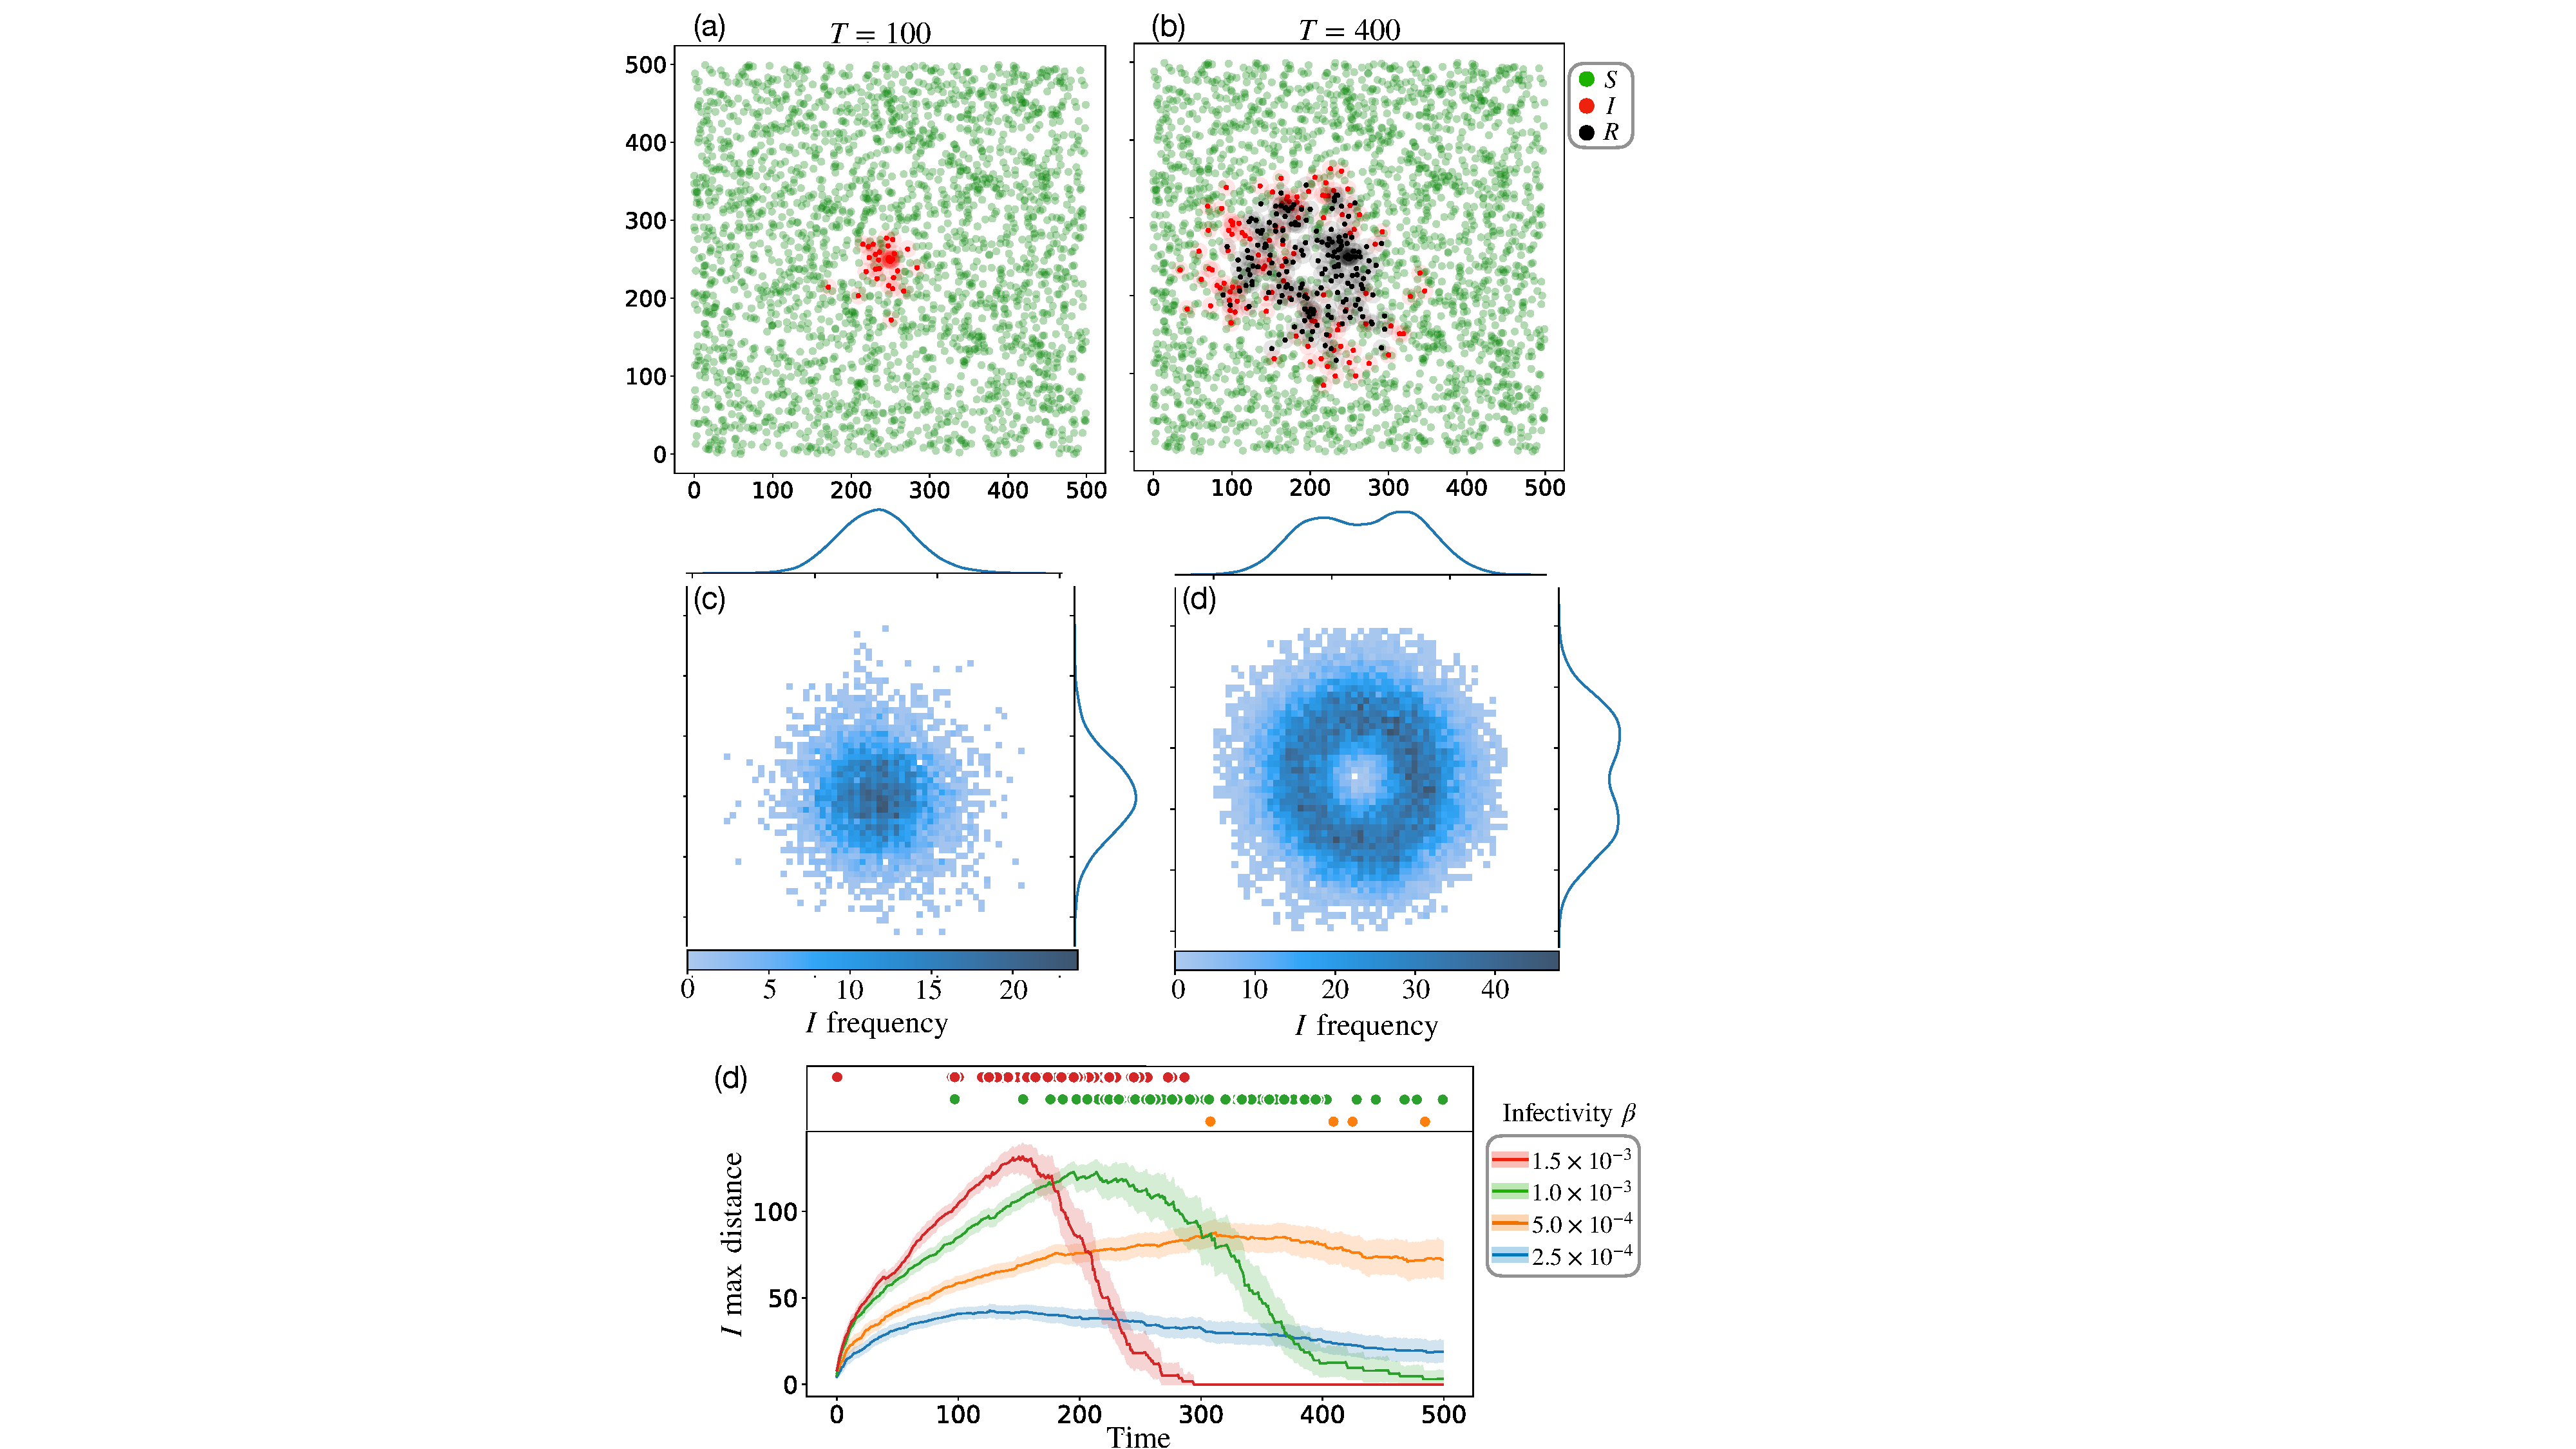
\includegraphics[scale=0.48]{chapter5/figures/fig1-sir-spatio-temporal.pdf}
    \caption{Spatio-temporal disease progression of the generic $SIR$ model with a small dispersal length scale of $\ell = 25$ and fixed density $\rho=0.01$. All figures were accessed in a domain of size $\mathcal{L} \times \mathcal{L} = 500 \times 500$. (a-b) An evolving epidemic with infectivity $\beta=1.0\times 10^{-3}$ is shown through two time-steps. Green pixels represent susceptible trees in $S$, while red pixels represent infected trees at different different steps in the $I$ category. Infected trees uniformly transition into the removed compartment at $t=100$, shown in black. (c-d) An ensemble-averaged spatio-temporal frequency distribution (of 200 repeats) representing the number of trees in the infected compartment. The probability of a infected tree located at row $x$ and column $y$ is represented by a KDE estimate in the upper and horizontal marginals. (d) The maximum infectious distance ensemble averaged over 100 repeats for epidemic parameters shown.}
\label{fig:sgm-evol}
\end{figure}

After $t$ time steps, the maximum distance reached by the pathogen is $D_{max}(t)$.
Figure \ref{fig:sgm-evol}(d) shows the ensemble averaged maximum infectious distance for four infectivity parameters.
\textcolor{red}{A $95\%$ confidence interval} is shown about the mean\textemdash shown as a solid line\textemdash for each time step.  % redo fig d with custom std   
The time-series indicates if the pathogen becomes extinct, or propagates to the lattice boundary and survives\textemdash marked by dots in the upper marginal plot for each infectivity parameter.
Survival to the boundary defines an effective cluster of infectious-removed trees spanning the domain, representing an epidemic.
On average, the highest value infectiviy propagates to the domain boundary first, demonstrated by comparing red and green line-plots.
In contrast, the pathogen fails to reach the domain boundary in the vast majority of simulation time-series shown in orange and blue
\textemdash barring the small number of rare samples shown in the upper marginal plot in orange.

Modelling the spread of disease for small $\frac{\ell}{\mathcal{L}}$ is useful to understand NLM, and presents a clear link to the percolation-based SLM.
However, a realistic, dispersal-based, tree disease is unlikely to exhibit the slow marching travelling wave at small spatial-scales\footnote{...reference landscape level fronts ~tenskm} that propagates through the domain. depicted in Figure \ref{fig:sgm-evol}.
In particular, as $\frac{\ell}{\mathcal{L}}$ becomes larger, the utility of tracking the maximum distance inside a finite domain of size $L$ becomes ill-defined 
as larger dispersal jumps can result.
Therefore, the time-series of $D_{max}(t)$ can dynamically capture the pathogen progressing through the domain when the scale of dispersal is small in comparison to the domain, but as we look to increase the scale of dispersal (ultimately to model wind-dispersal in chapter 6), an alternative metric is required to understand epidemic progression\textemdash
thus motivating a thorough examination of the reproductive ratio $R_0$ in section \ref{sec:spatially-explicit-reproduction-ration}.

\subsection{Normalising infectivity $\beta$}

Before we move onward, a tool to fix epidemic impact over various dispersal length-scales is outlined below.
Using $\beta$ to control infectivity in the model, as governed by equation \ref{eq:pr-dispersal-transition}, is pragmatic for single parameter of $\ell$\textemdash as shown in Figure \ref{fig:sgm-evol}.
However, suppose the dispersal parameter $\ell$ in equation \ref{eq:pr-dispersal-transition} is increased. 
Undoubtedly, more transitions into the $I$ compartment would result because the Gaussian kernel, $\exp\big[-r^2/(2\ell^2)\big]$, is unnormalised\textemdash effectively increasing the area under the kernel.
More secondary infections produced by each infected tree affords a more severe epidemic; in essence, infectivity (i.e. the strength of interaction between trees) in equation \ref{eq:pr-dispersal-transition} depends strongly on the scale of dispersal $\ell$ and epidemic-impact would vary greatly under different dispersal parameters.
This presents a challenge when accessing the model behaviour over different $\ell$ parameters.

To compare the model output over different $\ell$ parameters, the value of $\beta$ could be manually varied such that epidemic-impact is approximately matched between simulations\footnote{One may suggest that directly normalising the kernel poses a solution for matching the scale of epidemic for simulations with different $\ell$ parameters.
Although, this is ultimately incorrect from an implementation perspective. 
If the Gaussian kernel in \ref{fig:sgm-evol} is normalised, it would cease to be a yield a probability describing individual tree-to-tree interactions and the transition between states.}.
Undesirably, scaling $\beta$ differently for each $\ell$ parameter is cumbersome, and ultimately untenable for a large number of simulations.
A mathematical slight-of-hand can resolve the dilemma by simply factoring the dispersal normalisation factor out of $\beta$:
\begin{equation}
    \beta = \frac{\beta^*}{2\pi\ell^2}
    \label{eq:normalised-infectivity}
\end{equation}
where $\beta^*$ is an `auxiliary' infectiviy parameter that isolates infection pressure to a single parameter that remains fixed between simulations with different $\ell$ values.
In this manor, infectivity remains a probability $\beta=\beta^*/2\pi\ell^2 \in [0, 1]$ alongside the dispersal kernel $\exp\big[-r^2/(2\ell^2)\big] \in [0, 1]$, but importantly epidemic severity will be approximately matched\textemdash the limitations of this method are discussed below in section \ref{sec:spatially-explicit-reproduction-ration}.
So, henceforth, unless otherwise stated, the reminder of this chapter will employ the normalised infectivity\textemdash defined by the right-hand side of equation \ref{eq:normalised-infectivity}\textemdash will be substituted into equation \ref{eq:pr-dispersal-transition} to permit model comparisons over the parameter space of $\ell$.

\newpage

\subsection{SIR fitting: dispersal-mediated contact-mixing}

It is of practical interest to contrast the NLM against a well established, alternative model of epidemics.
Subsequently, the SIR model given by \cite{kermack-model} will be fitted to simulated data from the NLM.
Despite a static and spatially-structured host distribution, it makes sense to compare the NLM with predictions from the canonical SIR framework, given that the approach adopted so far pertains to the same compartmental dynamics $S \rightarrow I \rightarrow R$.

Two parameters control epidemic evolution in the SIR model, an infectiviy rate $\beta$ and removal rate $\gamma$. 
Both $\beta$ and $\gamma$ could be varied to see if the SIR equations yield similar results to a NLM simulation. Nevertheless, the task can be simplified significantly by considering $I$ as a function of $S$; this can be accomplished as follows:
\[
\frac{dI}{dS}=\frac{dI / dt}{dS /dt}= \frac{\beta IS/N - \gamma I}{-\beta IS/N} = -1 + \frac{\gamma}{\beta} \frac{N}{S} \]
Letting $\alpha = \frac{\gamma}{\beta}$ we have:
\[
    dI = \Big(-1 + \frac{\alpha N}{S}\Big)dS
\]
Now using integration by separation of variables:
\begin{equation}
\label{eq:SIR-1param}
     I = -S + \alpha N \ln (S) + C
\end{equation}
where $C$ is a constant of integration. Thus, we have reduced the task of trying to match two parameters to considering a single one, namely $\alpha$. Before we can fit the NLM to equation \ref{eq:SIR-1param} we need to determine $C$. Initially $S_0 + I_0 + R_0= N$ and $R_0=0$ i.e. $R_0$ is the number of removed at $t=0$, not the reproductive ratio. Thus, evaluating equation \ref{eq:SIR-1param} at $t=0$ gives:
\begin{align*}
I_0 + S_0 & = N \alpha\ln (S_0) + C\\ 
 \implies C &= N - N \alpha \ln (S_0) 
\end{align*}
Upon substitution back into equation \ref{eq:SIR-1param} we have:
\begin{equation}
\label{eq:SIR-1param1}
    I = -S + N\big(1 + \alpha \ln (S/S_0)\big)
\end{equation}
\textcolor{red}{more information on the behaviour of equation \ref{eq:SIR-1param} is given in the appendix...}
By fixing the initial conditions in the differential SIR equations to match the NLM simulations\textemdash i.e. with $I_0=1$ and $S_0=\rho \mathcal{L}^2$ \textemdash we can compare the NLM to the SIR model.

\textcolor{red}{As described in section \ref{ch2:lit-rev-compartmentalised-models}}, the canonical SIR model is non-spatial and rests on a `well-mixed' population assumption.
At first glance, contact mixing in the NLM can be anticipated to result from the interplay of dispersal, set by $\ell$, and the domain size, set by $\mathcal{L}$.
So, moving forward comparison with the SIR model will pay attention to the parameters $\ell$ and $\mathcal{L}$. Accordingly, Figure \ref{fig:SIR-fitting} shows the NLM fitted to equation \ref{eq:SIR-1param} for two domain sizes and two dispersal parameters.

In Figure \ref{fig:SIR-fitting}, data from the NLM ensemble mean is plotted in black alongside 25 repeated simulations shown in light blue; 
tree density is fixed to $\rho=0.01$ and the infectiviy is fixed to $\beta^*=4$, resulting in outbreaks above the epidemic threshold.
Using the least squares method\textemdash specially, the Levenberg-Marquardt algorithm \cite{more1978levenberg} implemented in Python\textemdash the ensemble mean was fitted to equation \ref{eq:SIR-1param}, shown in red.
In all panels, the arrow of time is from right to left i.e. initially the number of trees in $S$ starts high and decreases as the number of trees in $I$ rises then falls.
 
 \begin{figure}
    \centering
    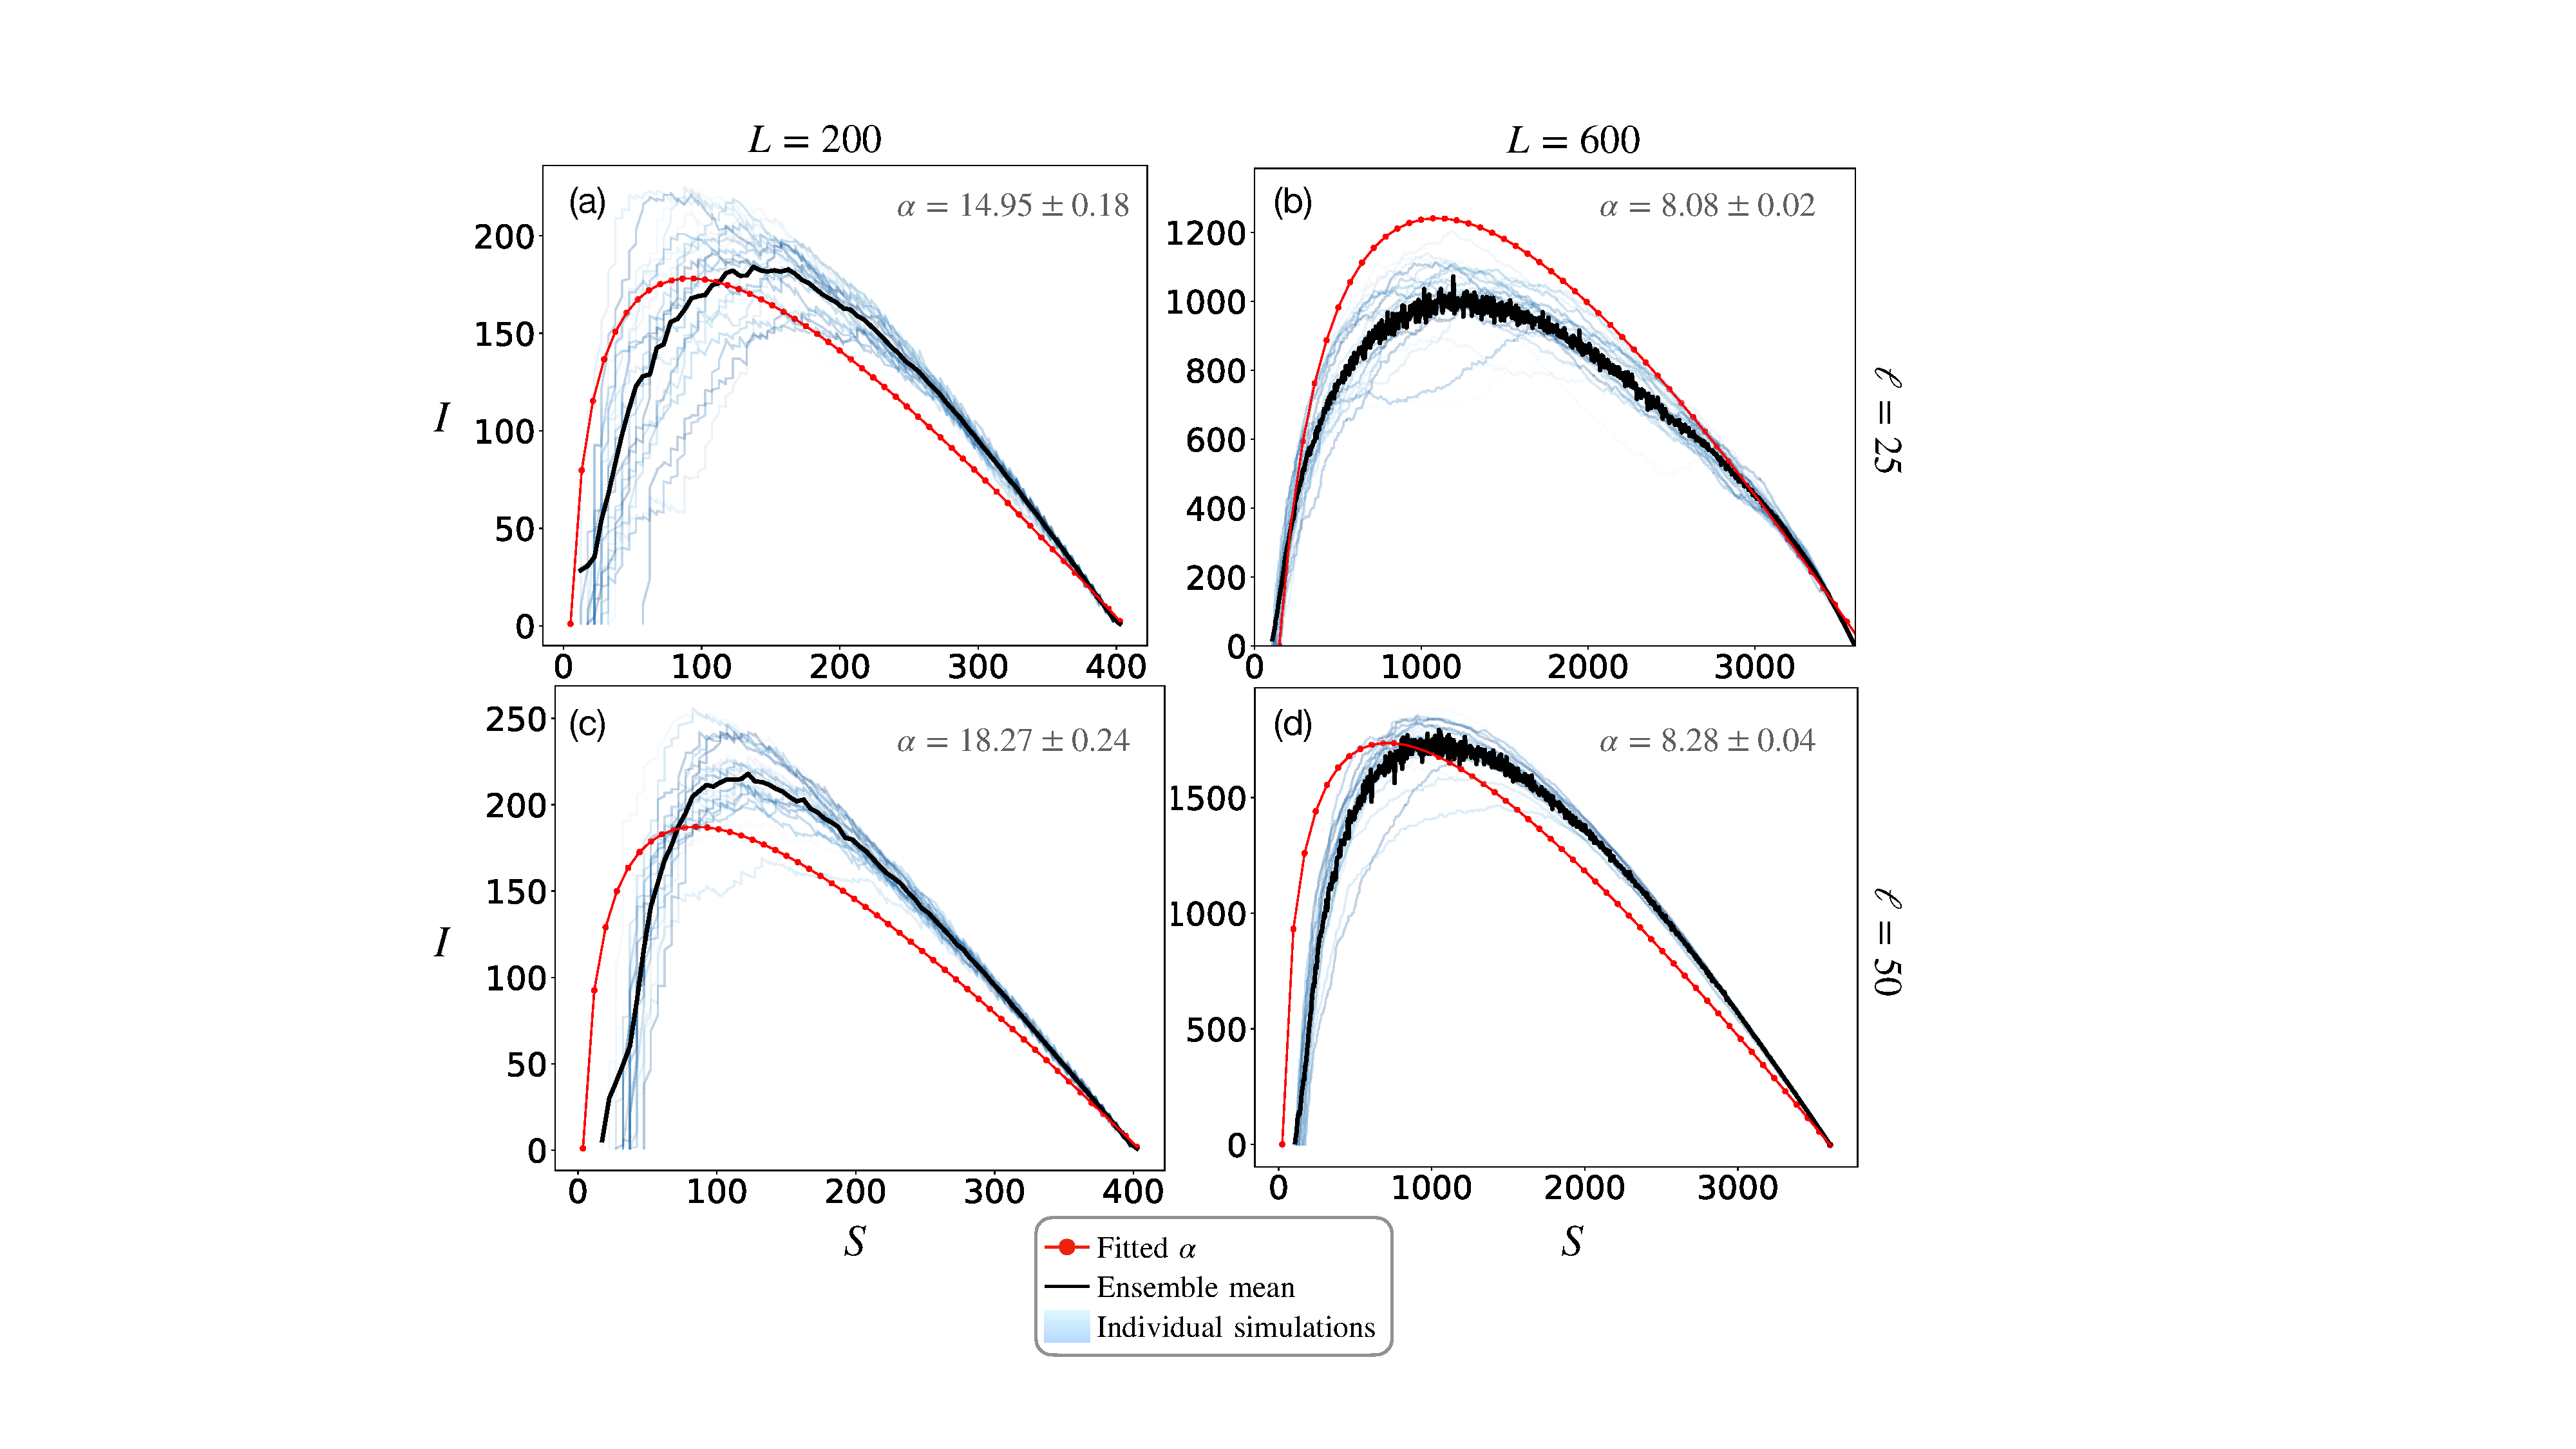
\includegraphics[scale=0.425]{chapter5/figures/fig2-sir-fitting-step.pdf}
    \caption{Fitting the non-local dispersal model (NLM) to the traditional $SIR$ model given by \cite{kermack-model}. All simulations evolved with parameters $\beta^{*}=4$ and $\rho=0.01$ above the threshold for spread. (a) A small localised dispersal kernel of $\ell=25$ fitted against the canonical $SIR$. On a small domain of size $200\times 200$, the NLM tends to spread faster that the fitted $SIR$ model. (b) On a larger patch of size $600\times 600$, the SIR model predicts a faster rate of spread in comparison to the NLM, illustrated by the disparity between red and black lines. (c) On $200\times 200$ sized domain, increasing the dispersal parameter to $\ell=50$ results in a similar trend to panel (b), albeit with slightly less agreement between NLM and SIR models. (d) Increasing the dispersal parameter to $\ell=50$ reduces the large disparity between SIR and NLM, shown in Figure (b).}
    \label{fig:SIR-fitting}
\end{figure}

 Interestingly, for all but one panel in Figure \ref{fig:SIR-fitting}, epidemics progress faster in the NLM than predicted by the SIR model\textemdash suggested by the NLM having a steeper gradient beginning from $S_0=\rho\mathcal{L}^2$. 
 One possible cause of disparity between models is due to infectious lifetime dynamics. 
 That is, exponentially-distributed life-times are implicit within the SIR model, in contrast, the NLM relies on uniform transitions into the $R$ compartment. 
As an example, take Figure \ref{fig:SIR-fitting}(a); at time $t=0$ 400 hosts are present in the domain and it takes precisely $t=100$ steps to elapse before the first transition into $R$.
On the other hand, trees evolving with SIR dynamics will gradually transition into into the $R$ compartment at all time steps according to an exponential distribution. 
For the same initial conditions, it follows that more infectious trees might be expected in the NLM between times\footnote{In appendix \ref{section:apendix_A}, Figure \ref{fig:SIR-fitting} is replicated, although equation \ref{eq:SIR-1param} was fitted against with exponential-distributed-variant of the NLM.
Consequently, Figure \ref{fig:SIR-fitting-expontial} in appendix \ref{section:apendix_A} shows, a closer fit to equation \ref{eq:SIR-1param}.} 
$t\in [0, T]$, leading to more secondary infections that, on average, increase the scale of epidemic.
 
Figure \ref{fig:SIR-fitting}(b) demonstrates another important aspect of NLM behaviour, related to contact mixing in the spatial host distribution.
Looking at Figure \ref{fig:SIR-fitting}(b), a faster rate of spread is predicted for the SIR model,
demonstrated the divergence between red and black lines.
In this regime, $\frac{\ell}{\mathcal{L}}$ in the NLM is small and contact-mixing in the host distribution can be assumed low \textemdash supported by Figure \ref{fig:sgm-evol} that demonstrated a wave-like spread. 
Moreover, divergence between models is reduced by increasing the dispersal parameter to $\ell=50$, illustrated in Figure \ref{fig:SIR-fitting}(d).
Figure \ref{fig:SIR-fitting} therefore indicates that if the system is approximately well-mixed, the NLM spreads comparatively to the SIR, albeit slightly skewed because of uniform life-time dynamics.
Whereas, if the system is not well-mixed a slower epidemic marches across the domain in a wave-like behaviour that deviates significantly from the SIR model.

Altogether, these results point toward the inability for non-spatial models, such as the $SIR$ model, to describe a spatially-structured model of tree disease. Although, in a parameter regime where the ratio $\ell / \mathcal{L}$ is sufficient for population mixing, the $SIR$ model can describe the system with some accuracy. 
Well-known results from percolation theory present a simple model to understand the observations of Figure \ref{fig:SIR-fitting}.
\textcolor{red}{Namely,...}.

% \item Link to literature on $SIR$ models, (spatial $SIR$?)... an investigation was undertaken to understand how the non-localised $SIR$ maps to traditional $SIR$ \cite{kermack-model}.
% \item Explain the simplified $SIR$-fitting method, of one parameter
% \item Figure \ref{fig:SIR-fitting} shows the simulated dispersal model fitted against the non-spatial $SIR$ model.
% \item For simulations with $\ell$ comparable to the domain size $L$, sufficient fitting was found to result. As $\ell$ is made smaller, localised spread results and the $SIR$ model predicts a much greater spread.
% \item when ell is small small compared to the domain, contact-mixing assumptions become invalid.
% \item Suggesting that for specific parameter/domain configurations non-spatial $SIR$-like methods can be employed. This has analogies to the metal-population model. 
% \item Although, when non-spatial models are employed locally in conjunction to 'between-patch' dispersal information is lost... link to research and here we are concentrating on small-scale epidemiology. 

\section{A spatially-explicit reproduction number}
\label{sec:spatially-explicit-reproduction-ration}

As remarked earlier, percolation-based distance metrics become ill-defined when the pathogen can jump on long distances.
Going forward, a more robust metric is required to examine the model.
To this aim, a basic reproduction number will be outlined for the NLM.
The concept of $R_0$ is widely used\textemdash and widely misinterpreted \cite{delamater2019complexity} \textemdash and different methods of calculating $R_0$ are available \cite{perspectives-on-r0}.
A thorougher review of the reproduction number, $R_0$ is undertaken in \textcolor{red}{ chapter 2}. Although, to recap, $R_0$ is fundamental to understand epidemic thresholds in human and animal populations. 

Various studies have considered $R_0$ for crop-based diseases 
\cite{gubbins2000population, park2001invasion, doi:10.1146/annurev.phyto.011108.135838, van2011periodic, mikaberidze2016invasiveness}.
Although, in the context of tree-based botanical diseases the concept remains less explored. 
In general, $R_0$ is complicated, and it may vary in response to various abiotic factors, such as temperature, humidity and wind-speed.
Furthermore, when defining an $R_0$ value for tree-disease, the importance of spatial structure cannot be
ignored \cite{park2001invasion}.
Importantly, any measure of $R_0$ should separate the regime of epidemic and confinement with a simple threshold condition i.e. defined by $R_0=1$.

\subsection{Analytically approximating $R_0$}

In this section, an idealised, spatially-explicit expression of $R_0$ is derived for the NLM.
Defining an informative $R_0$-value for tree-based pathosystems is not simple, and care is needed when defining an $R_0$ value. 
Beginning from simplicity, an `effective' reproduction number can be defined through the following thought experiment: 

\textit{Consider a single (primary) infected tree at time $t=0$, surrounded by a distribution of susceptible neighbouring trees. Over the course of it's infectious life-time, the primary infection will lead to $R_0$ secondary infections. If secondary infections do not in turn not produce other tertiary infections, the neighbourhood around the primary infection remains untouched by other diseased trees and the reproductive potential of the pathogen can be approximated by $R_0$. }

this scenario can be analytically approximated and numerically simulated in a straightforward manner, without the use of advanced mathematics.
Notwithstanding, the thought experiment is clearly idealised and spatial transmissions are likely to produce non-trivial spatial correlation in a homogeneous population of hosts\textemdash i.e. negative spatial correlations develop when the local density of susceptible hosts is reduced by other infected trees, discussed below.
The reader is referred to \cite{R0-perc-ref} for a useful discussion on $R_0$, heterogeneity and spatial correlations.

Suppose at time $t=0$ the domain is uniform with density $\rho_0$, and one singular infected tree exists inside a large domain.
In such a configuration, the mean number of secondary infections expected over the first time-step can be calculated by integrating equation \ref{eq:pr-dispersal-transition} as follows:
\begin{equation}
    R_0(t = 0) = \beta \rho_0 \int^{\infty}_{-\infty} \exp\Big(-\frac{r^2}{2\ell^2}\Big)dr= 2\pi\beta\rho_0\ell^2
\end{equation}
Assuming no host (re-)growth, less trees are available to infect at time-step $t+1$. 
Tee density can therefore be seen as a monotonically decreasing function of time $\rho(t)$, leading to the expression:
\begin{equation}
    R_0(t) = 2\pi\beta\ell^2\rho(t)
    \label{eq:r0-A}
\end{equation}
this expression presents a convenient relationship between tree density and the number of expected secondary infections. 
In a large, but finite, domain of size $\mathcal{L}$ tree density approximately follows:
\begin{equation}
\label{eq:drho/dt}
    \frac{d\rho}{dt} = - \frac{R_0(t)}{\mathcal{L}^2} = -\frac{2\pi\beta\ell^2\rho(t)}{\mathcal{L}^2}
\end{equation}
Solving the above, with initial condition $\rho_0$ at $t=0$, leads to:
\begin{equation}
\label{eq:rho(t)-linear}
    \rho(t) = \rho_0 \exp\Big(-\frac{2\pi\beta\ell^2}{\mathcal{L}^2} t \Big)
\end{equation}
Thus, after the infectious life-time of $T$ time-steps, the final number of expected secondary infections is given by:
\begin{equation}
\label{eq:Appendix_final_r0_approx}
    R_0(T) =  \mathcal{L}^2\big(\rho_0 - \rho(T)\big) = \mathcal{L}^2\rho_0\Big[1 - \exp\big(-\frac{2\pi\beta\ell^2}{\mathcal{L}^2} T \big) \Big]
\end{equation}

Note, for the purpose of transparency the above derivation is based on $\beta$ and not the normalised infectivity parameter. 
However, from equation \ref{eq:Appendix_final_r0_approx} it is clear to see how the normalised infectivity $\beta^*/2\pi\ell^2$ negates the influence of $\ell$ on the number of expected secondary infections.

Equation \ref{eq:Appendix_final_r0_approx} can be used as a first approximation toward an $R_0$ value.
Nonetheless, it implicitly assumes that secondary infections are equally likely at all spatial locations about the primarily infected tree\textemdash by virtue of uniform density reductions in equation \ref{eq:drho/dt}. 
Neglecting the spatial variation of expected secondary infections on average, overestimates the spread of disease.
A more accurate, albeit more complex, formula can be derived allowing for Gaussian spatial variations.

\subsection{Including spatial heterogeneity into $R_0$}

\label{sec:r0-derivation}
Equation \ref{eq:Appendix_final_r0_approx} neglects a spatially varying probability of transmission, 
but it can be refactored by first re-writing the density as:
\begin{equation}
\label{eq:rho(t)-ga-variations}
    \rho(r, T) = \rho_0\exp \big(-\beta T g(r; \ell) \big)
\end{equation}
where $g(r;\ell)$ is a Gaussian kernel. 
Equation \ref{eq:rho(t)-ga-variations} can be interpreted as the generalised form of equation \ref{eq:rho(t)-linear}, this time incorporating Gaussian spatial variations into $R_0$.
Upon substitution back into equation (\ref{eq:Appendix_final_r0_approx}), the total number of secondary infections after $T$ time-steps is given by:

\begin{equation}
\label{eq;R0(t)-ga-variations}
   R_0(T) = \int ^\infty _0 2\pi r \big (\rho_0 - \rho(r, T)\big)dr =  \int ^\infty _0 2\pi r \rho_0 \Big[1 - \exp\big(-\beta T g(r;\ell)\big) \Big]dr
\end{equation}

Note, the finite lattice square of size $\mathcal{L}^2$ has been replaced with integration in polar coordinates over $dr$. 
Equation \ref{eq;R0(t)-ga-variations} is hard to solve directly, but it can be integrated by performing a series expansion on the exponential term. 
One may then proceed to integrate on a term-by-term basis:
\begin{equation} 
\label{eq:Appendix_final_expression}
\begin{split}
R_0(T) & = \int^\infty_0 2\pi r \rho_0 \Big[1 - \exp \big( -\beta T g(r;\ell)\big)\Big]dr \\
& = 2\pi\rho_0 \int^\infty _0 r \Big[1 - \sum^\infty_{n=0} \frac{\big(-\beta T)^n}{n!} \exp\big(-\frac{r^2}{2\ell^2}\big)^n  \Big] dr \\
& = 2\pi\rho_0 \int^\infty _0 r \Big[\sum^\infty_{n=1} \frac{(-1)^{n+1}\big(\beta T)^n}{n!} \Big(\exp(-\frac{n r^2}{2\ell^2} ) \Big)  \Big] dr \\
& = 2\pi\rho_0 \sum^{\infty}_{n=1} \frac{(-1)^{n+1} (\beta T)^n}{n!} \int^\infty _0 r \exp(-\frac{n r^2}{2\ell^2})dr  \\
& = 2\pi\rho_0 \ell^2 \sum^{\infty}_{n=1} \frac{(-1)^{n+1}(\beta T)^n}{(n)(n!) }
\end{split}
\end{equation}

if $\beta$ and $T$ are small, the $1^{st}$ order term in equation \ref{eq:Appendix_final_expression} is sufficient to approximate $R_0$ as a linear function of $T$\textemdash
confirmed by numerical simulations in the next section. 
Finally, equation \ref{eq:Appendix_final_expression} can be summed to give:
\begin{equation} 
\label{eq:Appendix_final_expression1}
\begin{split}
R_0(T) & = 2\pi\rho_0 \ell^2 \sum^{\infty}_{n=1} \frac{(-1)^{n+1} (\beta T)^n}{(n)(n!)}\\
& =  2\pi\rho_0 \ell^2 \big(E_1(\beta T) + \ln (\beta T) + \gamma\big)
\end{split}
\end{equation}
where the function $E_1(x)$ is the mathematically well studied exponential function $E_1(x)=\int^{\infty}_x t^{-1}\exp^{-t}dt$ and $\gamma$ is the Euler–Mascheroni constant $\approx 0.57721$.
Intriguingly, the jump between equations \ref{eq:Appendix_final_expression} and \ref{eq:Appendix_final_expression1} is well known in the field of complex analysis\textemdash see \cite{abramowitz1948handbook}, page 228.
Alternatively, the summation in equation \ref{eq:Appendix_final_expression} could equivalently be given as:
\begin{equation}
\label{eq:ein}
     \mathrm{Ein}(\beta T) = \sum^{\infty}_{n=1} \frac{(-1)^{n+1} (\beta T)^n}{(n)(n!)}
\end{equation}
where $\mathrm{Ein}$ is known as the `entire' function, leading to the well established relation:
\[
E_1(z) = -\gamma - \ln(z) + \mathrm{Ein}(z)
\]
The next section will investigate the suitability of \ref{eq:Appendix_final_expression1} to describe the NLM.

\section{Analytic behaviour of $R_0$}

% R0 can be calculated from experimental data : \cite{segarra2001epidemic}
% \label{ch5:dispersal-model}
\begin{figure}
    \centering
    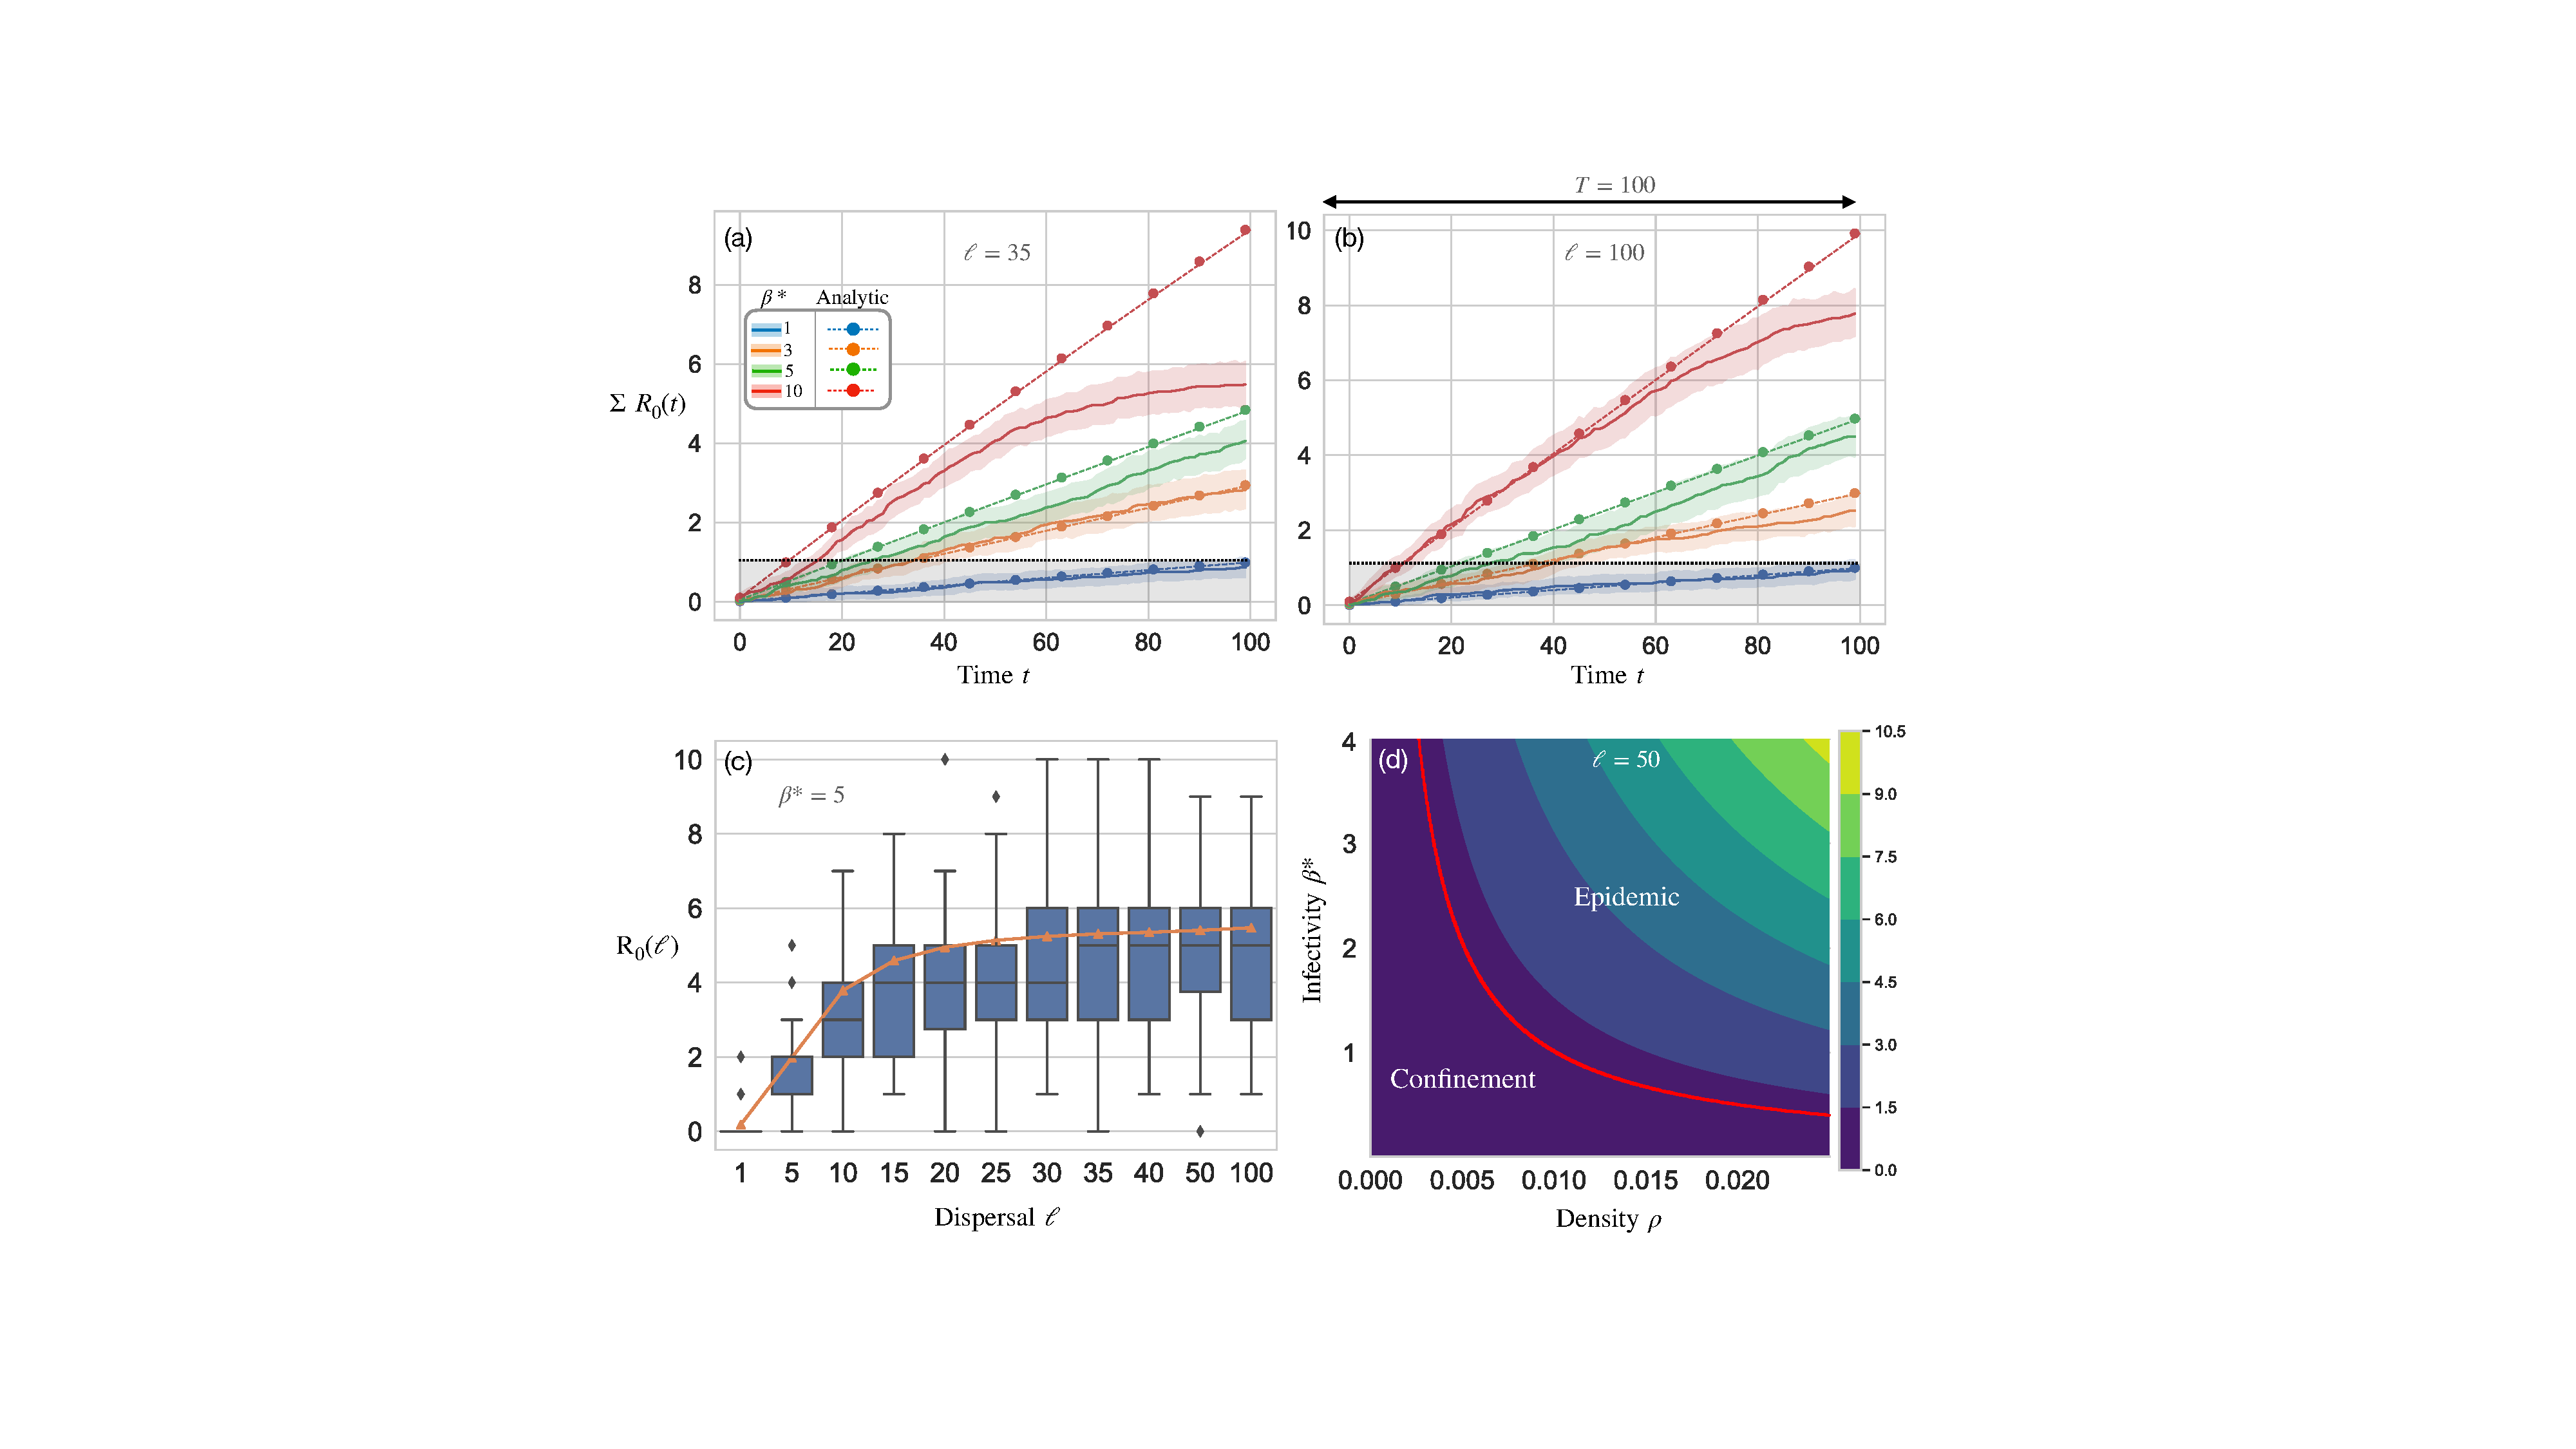
\includegraphics[scale=0.40]{chapter5/figures/fig3-R0-analytic.pdf}
    \caption{Comparisons between the analytical expression for $R_0$, according to equation \ref{eq:Appendix_final_expression1}, and NLM simulations. (a) For a small dispersal value of $\ell=10$ and high infectivities (indicated by color), $R_0$ begins to saturate to a maximum over the infectious period. Whereas, for smaller values of infectivity, $R_0$ increases at a constant rate and fails to saturate\textemdash reflected in purple-red. (b) For a larger dispersal kernel, $R_0$ increases at a constant rate for all infectivities, linearly increasing over the infectious period. (c) $R_0$ is shown as a function of the dispersal parameter for a fixed infectivity $\beta^*$. For small length scales, the normalised infectivity produces a less infectious outbreak. However, $R_0$ is approximately fixed for larger $\ell$ values. (d) The 2D $R_0$ phase plane predicted by equation \ref{eq:Appendix_final_expression1}. A threshold, given by $R_0=1$, is plotted in red and predicts the separation between confinement and epidemic.}
    \label{fig:my_label}
\end{figure}

The idealised reproduction number, as discussed above and described by equation \ref{eq:Appendix_final_expression1}, is compared against NLM simulations\footnote{Implementing a comparative test between NLM simulations and equation \ref{eq:Appendix_final_expression1} was straight forward, and only required one minor tweak in the program dynamics. Simply put, when the primary infected tree produces a secondary infection it transitions straight into the removed compartment. Owing to the single infected tree in $I$, simulations were computationally efficient and ensemble-averaged results could be generated in good time.} in Figure \ref{fig:R0-vs-NLM-sims}.
Stochasticity within the NLM required an ensemble of size $10^3$.
Figure \ref{fig:R0-vs-NLM-sims}(a) shows the ensemble-averaged number of secondary infections determined at each time-step $t\in [0, T]$, plotted as a time-series $R_0(t)$.
The ensemble average is depicted as the solid line and continuous error bars are shown by the shaded regions.
The time-series in Figure \ref{fig:R0-vs-NLM-sims}(a) show four variations of $\beta^*$ alongside the dotted curves predicted by equation \ref{eq:Appendix_final_expression1} for a small dispersal kernel of $\ell$. 
The final value of $R_0$ is observed when the infectious life-time of $T=100$ steps is concluded. 

Lower infectivity values in Figure \ref{fig:R0-vs-NLM-sims}(a), shown from purple-green, approximate a linear relationship which agrees well with equation \ref{eq:Appendix_final_expression1}.
Here, linearity reflects a constant transition rate into the $I$ compartment as the neighbourhood fails to become saturated with infected trees. 
For progressively higher infectivities the number of secondary infections begin to plateau as less trees in the neighbourhood are available to infect.
For particular high values of $R_0$, equation \ref{eq:Appendix_final_expression1} begins to deviate from model output, reflecting the inability of equation \ref{eq:Appendix_final_expression1}
to describe highly infectious outbreaks.

In Figure \ref{fig:R0-vs-NLM-sims}(b), the dispersal parameter is increased to $\ell=50$.
A larger dispersal kernel encompasses a larger neighbourhood.
Subsequently, $R_0(t)$ does not saturate/plateau for higher $R_0$ values, in contrast to Figure \ref{fig:R0-vs-NLM-sims}(a).
Indeed, despite a surprising degree of simplicity, the linear relation is predicted by equation \ref{eq:Appendix_final_expression1}.
The linearity can be understood by noting that when $\mathrm{Ein}(\beta T)$ is small in comparison to $\ell^2$ (and $\beta T$ is small), the first order term inside equation \ref{eq:Appendix_final_expression1} reduces to a linear equation in $T$.
More interestingly however, we can observe that $R_0$ is similar when $\beta^*$ is low\textemdash c.f. the purple lines between Figures \ref{fig:R0-vs-NLM-sims}(a-b).
Whereas, for higher infectivities $R_0$ tends toward a smaller value in Figure \ref{fig:R0-vs-NLM-sims}(a) comparison to panel (b).
Observing $R_0$ deviate with different $\ell$ parameters compels a study of $R_0$ over the space of $\ell$, which leads to Figure \ref{fig:R0-vs-NLM-sims}(c).

In Figure \ref{fig:R0-vs-NLM-sims}(c), the basic reproduction number $R_0$ is assessed over a range of dispersal kernels.
Tree density in Figure \ref{fig:R0-vs-NLM-sims}(c) is fixed fixed to $\rho=0.01$ together with a high infectivity of $\beta^*=10$.
Predictions from equation \ref{eq:Appendix_final_expression1} are shown in orange;
$R_0$ can be seen to increase with the dispersal kernel up to around $\ell \in [25, 30]$ before saturating to $R_0 \approx 10$. 
These observations indicate that neighbourhoods defined by a small $\ell$ parameter are likely to become fully occupied by secondary-infected trees, resulting in a lower $R_0$.
Then, as one increases the kernel, $R_0$ asymptotically increases to a maximum value beyond which increasing $\ell$ bares no impact on $R_0$\textemdash provided that the number of secondary infected trees is small in comparison to the number of hosts in inside the neighbourhood\footnote{Insight into the underlying behaviour could be gleaned by looking at equation \ref{eq:Appendix_final_expression1}. That is, by accessing the growth of $2\pi \rho_0 \ell^2$ and the convergence of the function $\mathrm{Ein}$ (defined by equation \ref{eq:ein}) and noting that as $\ell \rightarrow \infty$, $\beta=\beta^*/2\pi\ell^2 \rightarrow 0$. Although an in-depth mathematical analysis was not undertaken, it is clear that for large values of $\ell$, $R_0$ asymptotically approaches a limiting value.}.
Therefore, if $\ell$ is large enough, the normalised infectivity can be seen to effectively constrains the epidemic severity to a limiting value.

From the reproduction number, a transmission threshold can be defined by $R_0=1$,  predicting the separation of states, between confinement and epidemic.
In Figure \ref{fig:R0-vs-NLM-sims}(d), the threshold predicted by equation \ref{eq:Appendix_final_expression1} is marked in red, overlaying a two dimensional phase plot of $R_0$ over tree density and infectivity.
According to Figure \ref{fig:R0-vs-NLM-sims}(d), when model parameters satisfy $R_0>1$, the pathogen may propagate for a time before dying off or culminate in a epidemic;
for $R_0<1$, the pathogen has little chance of spreading to neighbouring trees and little to no chance of causing a large-scale epidemic.
In theory, equation \ref{eq:Appendix_final_expression1} provides a computationally efficient means to categorise model behaviour.
However, given its idealised nature, it remains to be seen how well equation \ref{eq:Appendix_final_expression1} correlates to the final epidemic state final-sized epidemic, the likelihood of $R_0>1$ causing an epidemic, or indeed whether a threshold is realised in practice.

\subsection{Tree mortality versus $R_0$}

Ideally, one should also be able to predict the final outcome based on observations of the first few infectious cases. 
For a well-mixed homogeneous population, the reproduction number can be used to estimate the number of expected cases as a fraction of the population.
In the standard SIR model, this is given by:
\begin{equation}
\label{eq:final-sized-epi}
    R_{\infty} = S_0\Big[]1 - \exp\big( R_0 R_\infty\big) \Big]
\end{equation}
where $R_\infty$ is the number of cases as a fraction of the population size (the so called `final-sized epidemic'). 
When there is spatial structure, as in the NLM, the relation given by equation \ref{eq:final-sized-epi} would no doubt be more complex.
In this section, we therefore investigate predictions from the analytic $R_0$ and the number of host removals during the course of a simulation.
This investigation is further compelled by the fact that multiple methods can be used to calculate $R_0$, and ideally, methods should be accompanied by evidence that it defines a threshold
\cite{li2011failure}.

Varying both $\rho$ and $\beta^*$ results in a different $R_0$ prediction.
In this way, $R_0$ predictions can be plotted against the total number of hosts transitioning into the $R$ compartment\textemdash labelled as `tree mortality' in chapter \ref{fig:ch4_uk_spread}.
In Figure \ref{fig:R0-vs-NLM-sims}(a), ensemble-averaged tree mortalities are plotted as a function of the predicted $R_0$ value for three variations of tree density $\rho$, indicated by the solid blue-green lines.
Simulations were repeated in an ensemble of size $250$, and each individual simulation evolved until all infected tree became extinct or for $2500$ time-steps elapsed, whichever occurred first.
The ensemble-averaged mortality is overlaid by a scatter plot depicting a small sample of data points, the color of each sample point reflects the infectivity parameter $\beta^*$.

\begin{figure}
    \centering
    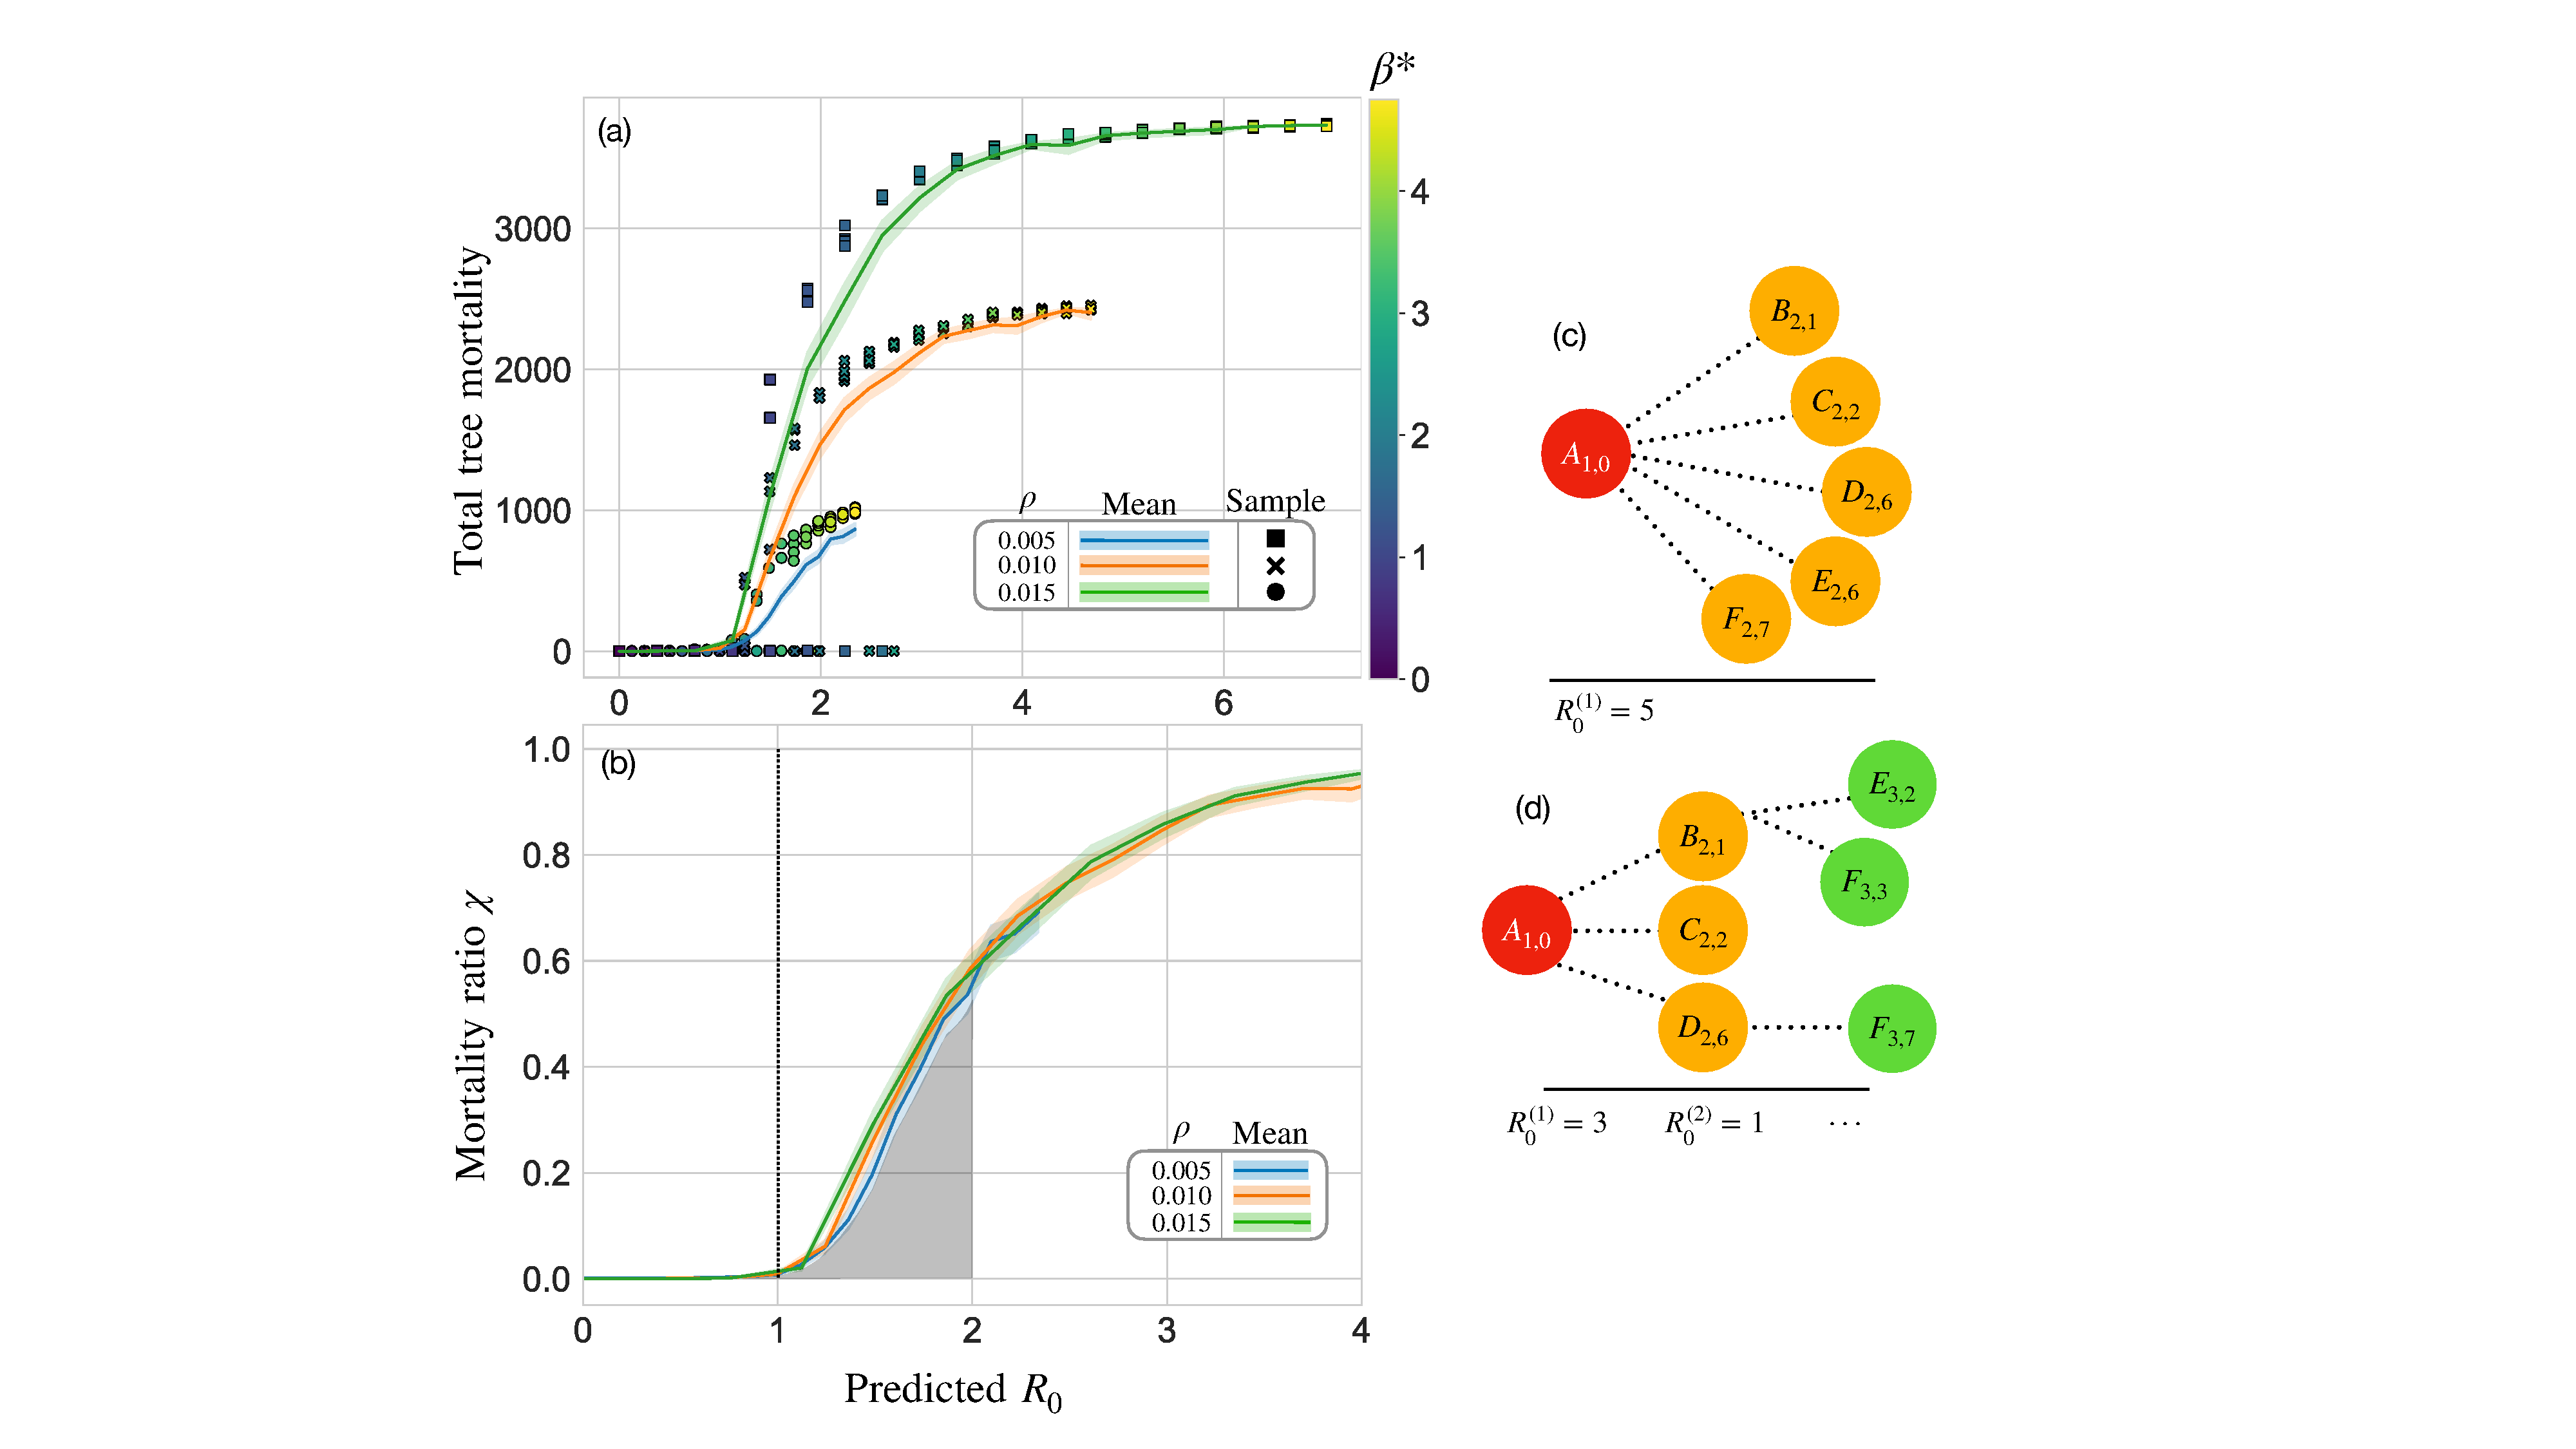
\includegraphics[scale=0.44]{chapter5/figures/fig4-R0-analytic-vs-mortality.pdf}
    \caption{The relationship between the total tree mortality and predicted $R_0$ value. (a) For three values of tree density, and numerous infectivity values, the ensemble-averaged tree mortality (as continuous solid line) is overlaid with a small sample of data points shown by the scatter plot. The shape and color of each data point indicates the tree density and infectivity respectively. (b) The fraction of removed trees as a fraction of the population is plotted against mortality the analytical value of $R_0$. Together panels (a) and (b) demonstrate a threshold-like behaviour at $R_0=1$. (c) A graphical representation of the idealised network and method of calculating $R_0$, as per equation \ref{eq:Appendix_final_expression1}. (d) A more realistic `branching process' representation of the spread of disease. In both (c) and (d) the arrow of time is from left to right and subscripts reflect the generation and time-step that trees become infected.}
    \label{fig:R0-vs-NLM-sims}
\end{figure}

According to Figure \ref{fig:R0-vs-NLM-sims}(a), when $\beta^*$ is low the reproduction ratio satisfies $R_0<1$ and tree mortality is kept low.
Additionally, when the infectivity is increased such that $R_0>1$, a large rise in mortality can be seen.
Equation \ref{eq:Appendix_final_expression1} therefore demonstrates a threshold-like behaviour defined by $R_0=1$.
Above the threshold $R_0=1$, increasing the tree density increases the scale of epidemic because more susceptible hosts are available to infected\textemdash indicated by a larger rise in tree mortality in green.

Despite being above the threshold, simulations can still fail to produce an epidemic,
illustrated by the small number of data points beyond $R_0=1$ that map to a zero-sized epidemic e.g. at $R_0\approx 2$ a small number of points can far below each ensemble mean.
In a similar vein, the ensemble mean is slightly lowered by simulations that fail to produce an epidemic\textemdash demonstrated by the small difference between the collection of points and the ensemble mean in the interval $R_0 \in [1, 3]$.
These observations result from the fact that under the influence of early stochastic forces the probability of epidemic extinction is higher \cite{perspectives-on-r0, R0-perc-ref} which unfortunately mark a flaw in the concept of $R_0$ as a general concept \cite{li2011failure}.

Figure \ref{fig:R0-vs-NLM-sims}(b) presents the same essential information as Figure \ref{fig:R0-vs-NLM-sims}(a).
Although, the ensemble mean is plotted against the mortality ratio (i.e. the total number of removed trees as a fraction of the total population), denoted by $\chi$.
Given that each ensemble mean converges to the same effective epidemic scale, the quantity $\chi$ demonstrates utility when accessing the epidemic impact between different tree-densities.
Consequently, the threshold $R=1$ is easily observable in Figure \ref{fig:R0-vs-NLM-sims}(b), indicated in shaded grey.
The threshold-like behaviour witnessed in Figures \ref{fig:R0-vs-NLM-sims}(a-b) demonstrate that equation \ref{eq:Appendix_final_expression1} provides a simple predictive framework for the  NLM.
That being said, more complicated dynamics\textemdash such as exponential life-times, elaborate dispersal kernels or host aggregation\textemdash could significantly hinder the analytic solution proposed in section \ref{sec:r0-derivation}.

Another limitation to the equation \ref{eq:Appendix_final_expression1} can be explained by Figure \ref{fig:R0-vs-NLM-sims}(c), which shows a typical NLM simulation used to access the analytic expression of $R_0$.
Namely, a single `fist-generation' infected tree at time $t=0$ ($A_{1, 0}$) that happens to infect a number of neighbouring trees ($B_{1,1}$ to $G_{1, 7}$).
According to the $R_0$ approximation, the local density reductions due to $B_{2,1}-G_{2, 7}$ are neglected and $A_{1, 0}$ remains the only active source of infection.
Neglecting the influence of other secondary infected hosts helped to keep analytical derivation simple.
But for highly infectious outbreaks, equation \ref{eq:Appendix_final_expression1} is likely to overestimate $R_0$.
Figure \ref{fig:R0-vs-NLM-sims}(d) can be used to understand why overestimates of $R_0$ are likely.
In Figure \ref{fig:R0-vs-NLM-sims}(d), non-trivial density reductions could be expected from the second and third generation of infected hosts, $B_{2,1}, C_{2, 2}, D_{2, 6}$ and $E_{3 2}, D_{3, 5}, D_{3, 6}$ respectively\textemdash here, the first subscript refers to time and the second subscript refers to the generation\textemdash 
leading to an environment where the primary infected host $A_{1, 0}$ has less neighbours to infect.
Given these potential limitations, an improved, more flexible, method of calculating $R_0$ is investigated in the next section.

\section{Contact-tracing $R_0$: a computational approach}

% reference for network model of secondary infections \cite{PAUTASSO2010424} r
In this section an alternate method of calculating $R_0$ is presented that incorporates the effect of secondary infections  
(up the $n^{th}$ generations), analogous to contact-tracing emerging epidemics in human populations \cite{eames2003contact}.
By collecting individual tree-to-tree induced secondary infections the entire history is captured, illustrated graphically in Figure \ref{fig:R0-vs-NLM-sims}(d).
At $t=0$ the first generation primary infected tree, denoted by $A$, produces three $2^{nd}$ generation infections $B$-$D$ in orange that in turn produce
third generation infections shown in green.
The contact-traced $R_0$ can be defined by:
\begin{defn} % look into definitions of next-generation operator
\label{def:R0_contact_traced}
Beginning from one or more primarily infected trees at time $t=0$, the entire epidemic history is record to know which host infects which others.
The mean number of secondary infections that result for each generation $i$ is computed and denoted by $R^{(i)}_0$.
\end{defn}
to achieve this, trees are treated as particles in the sense that individual interactions between them are computed\textemdash discussed more below.

\begin{figure}
    \centering
    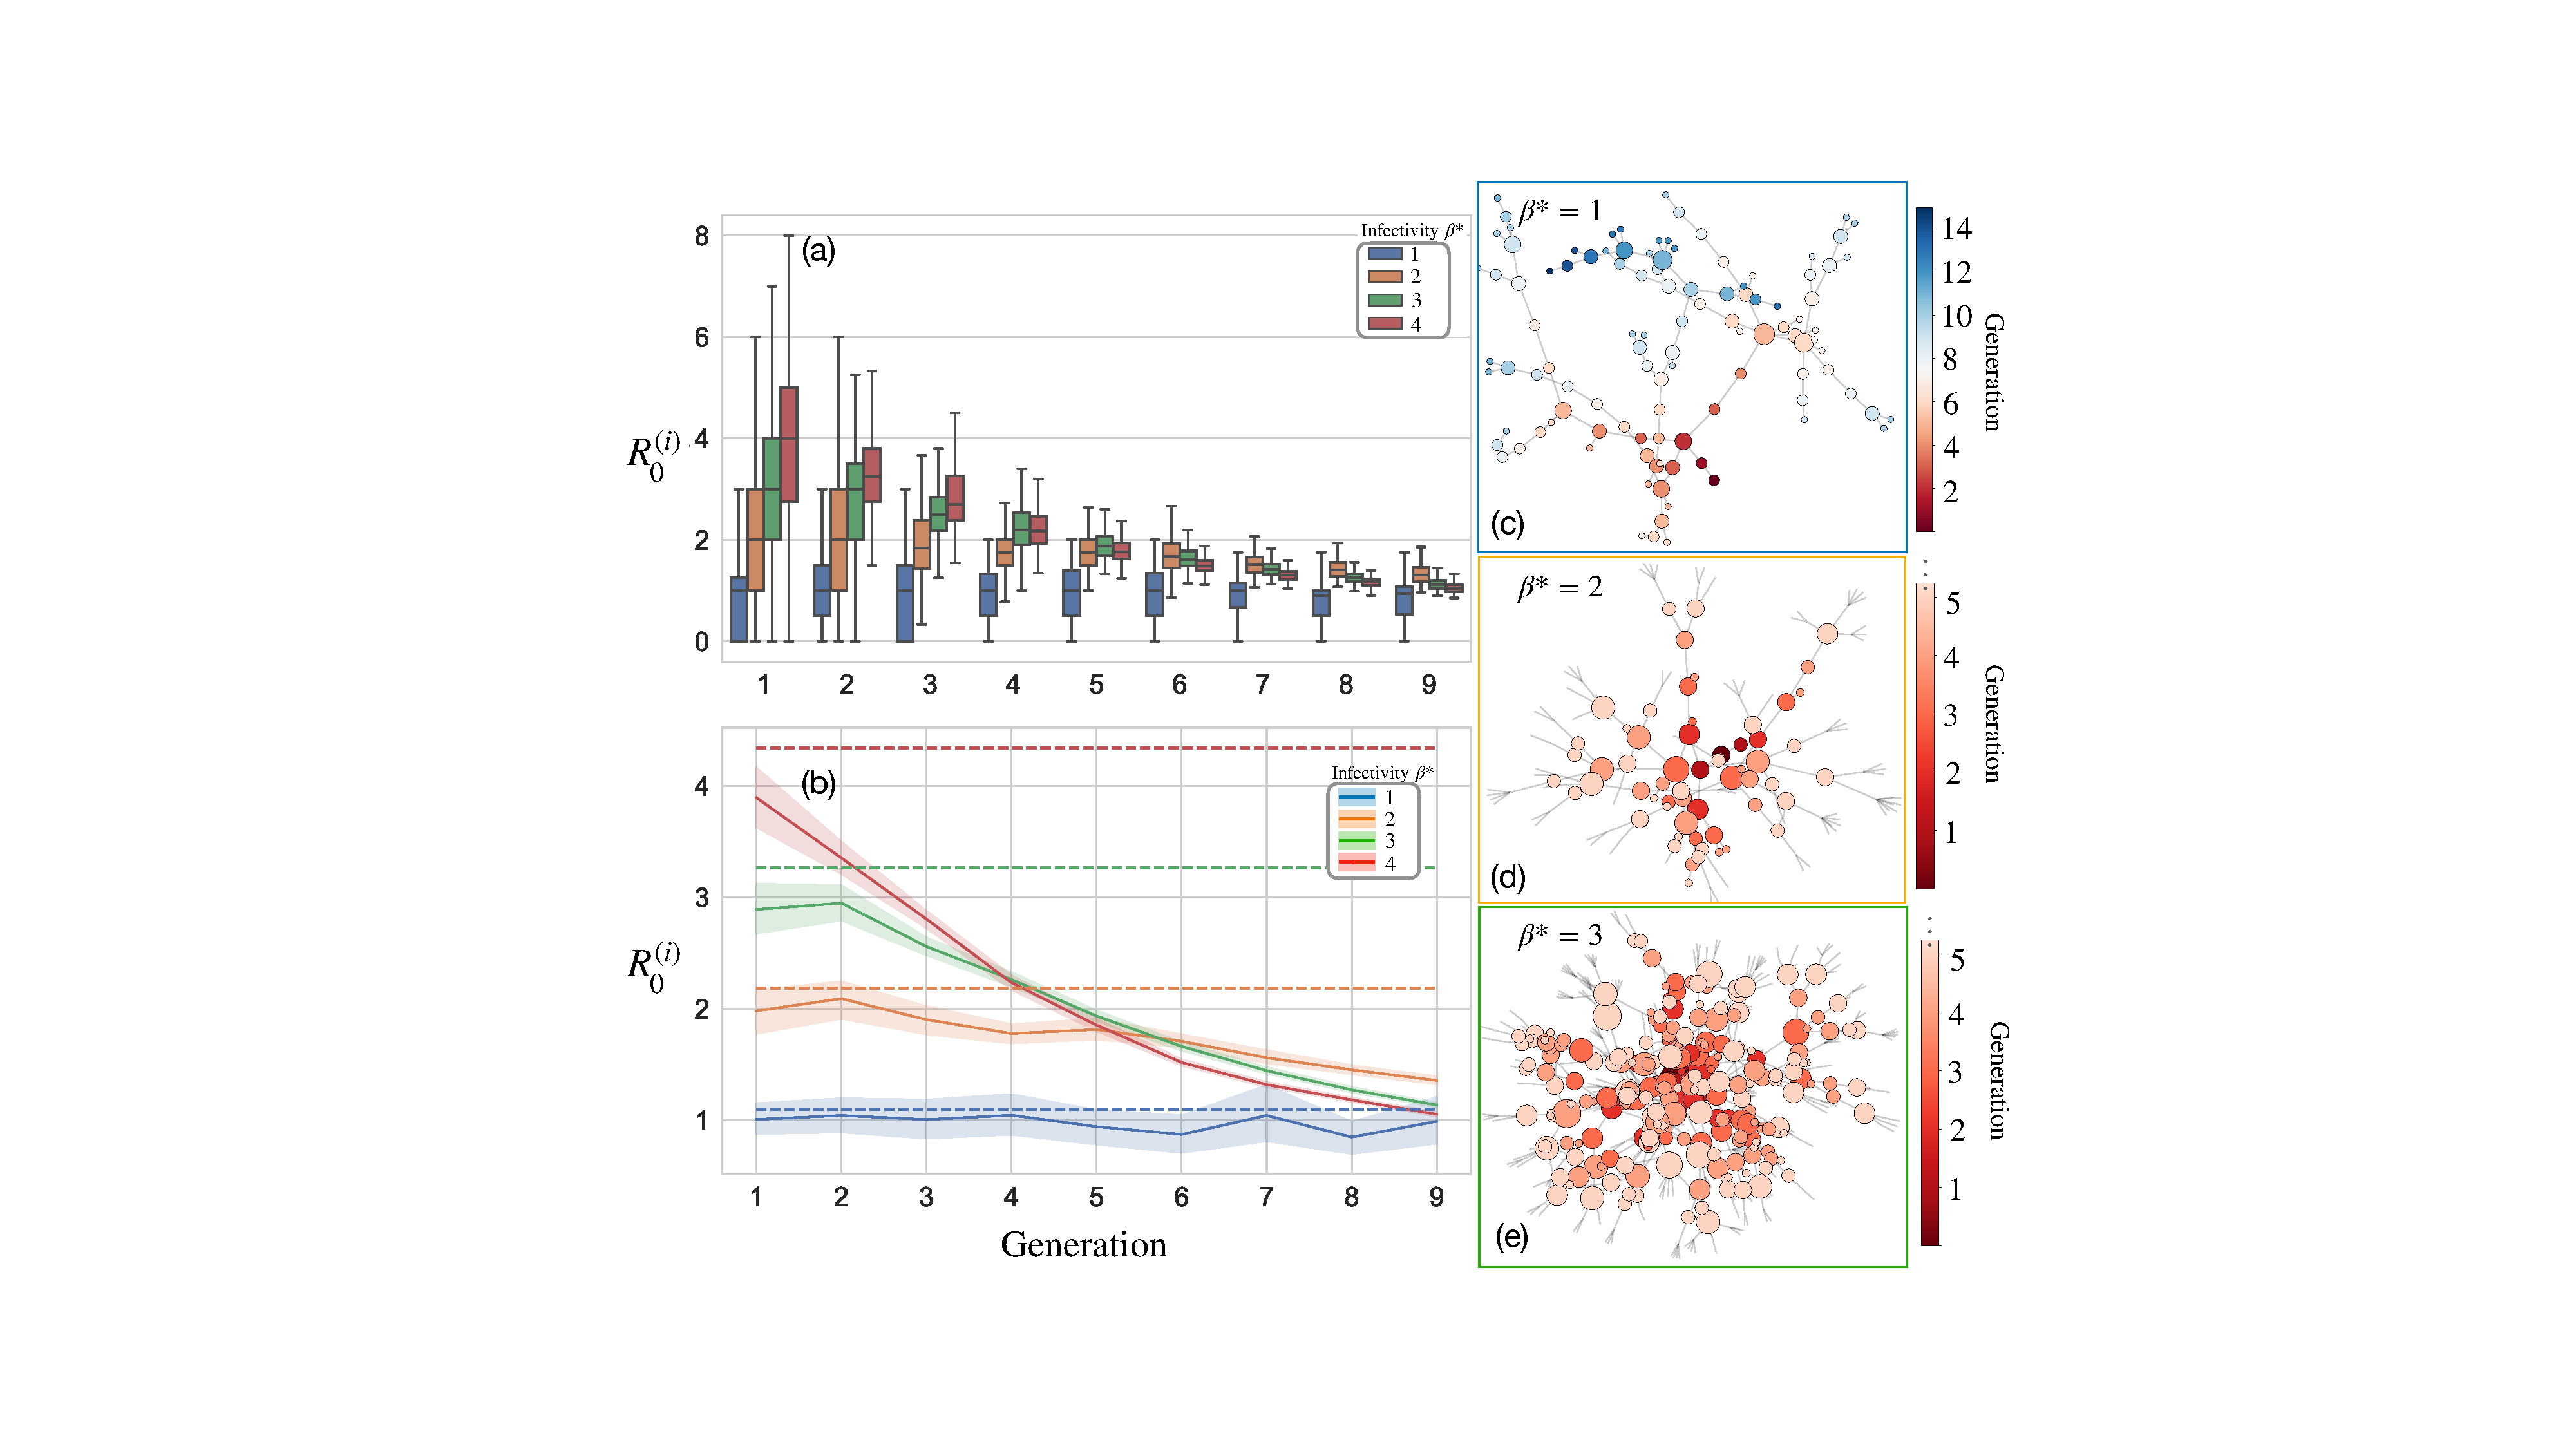
\includegraphics[scale=0.475]{chapter5/figures/fig5-R0-contact.pdf}
    \caption{Contact-tracing mean number of secondary infections for the $i^{th}$ generation of infected trees, $R^{(i)}_0$. For all simulations, tree densities are fixed along with dispersal kernels, ($\rho=0.01$) and $\ell=50$ respectively, inside a domain of size $\mathcal{L \times L} = 500 \times 500$.
    (a) A box and whisker plot showing mean number of secondary infections plotted over $10$ generations over an ensemble of size $N=500$. Four different infectivity values are shown from blue to red. (b) The ensemble-mean of panel (a) is compared against predictions from the analytic expression of $R_0$, plotted as horizontal dashed lines. For early generations, equation \ref{eq:Appendix_final_expression1} agrees well with the contact-traced value of $R_0$ but overestimates the spread for higher infectivities. (c-e) A network diagram representation of typical simulations for parameters $\beta^* \in \lbrace 1, 2, 3 \rbrace $. The color and size of nodes reflect the generation of infection and the number of secondary infections respectively.}
    \label{fig:contact-trace}
\end{figure}

In Figure \ref{fig:contact-trace}(a), observations from the (ensemble-averaged) contact-traced $R_0$ is shown for $10$ generations and 
four infectivity parameters; in all plots, tree densities, dispersal kernel and domain sizes remain fixed ($\rho=0.01, \ell=50, \mathcal{L}=500$).
For highly infectious outbreaks, the host population quickly decreases and $R^{(i)}_0$ begins high and gradually decreases with each generation.
In contrast, for infectivities just above the threshold $R^{(i)}_0$ remains approximately stable with each generation because the population of susceptible hosts remains high.  
For all boxes in Figure \ref{fig:contact-trace}(a), the interquartile range decreases with generation, suggesting that early stochastic forces increase the spread of $R^{(i)}_0$ values.
The number of secondary-infected trees will therefore vary over time and mirror the host population.
Had the re-growth of susceptible trees been considered, $R^{(i)}_0$ can be speculated to behave very differently for later generations.
In addition, variations in $R^{(i)}_0$ could, in theory, be strongly influence the domain boundary i.e. centrally located trees are likely to have more susceptible neighbours than trees located on the edge of the domain.

% 1) Here $R_0$ is just above threshold for earlier times and barely spreads, however, the spread is chaotic. %
% 2) From Figures \ref{fig:contact-trace}(b-d), we have demonstrated that this definition of $R_0$ %
% reliably captures the threshold of transmission during the initial stage of infection. %
% Undesirably, we have made simplification in the assumptions and have not achieved a complete %
% characterisation of $R_0$\textemdash which could, in be defined in terms of a growth %
% rate per generation \cite{R0-construct}. %

Figure \ref{fig:contact-trace}(b) compares the ensemble-averaged $R^{(i)}_0$ values, shown in Figure \ref{fig:contact-trace}(a),
to predictions from the analytic expression for $R_0$.
Analytic $R_0$ values are plotted as horizontal dashed lines and each ensemble mean is shown as solid lines surrounded by shaded bounds reflecting a $95\%$ confidence interval.
For the lowest infectiviy parameter around the threshold $R^{(i)}_0=1$, shown in blue, the contact-traced value of $R_0$ compares well with equation \ref{eq:Appendix_final_expression1}.
However, increasing the infectivity to $\beta^*=2$ (in orange) equation \ref{eq:Appendix_final_expression1} agrees well for early generations, but deviates for later generations, 
revealed by comparing the dashed horizontal and solid orange lines.
Deviations only grow larger as $\beta^*$ increases.
That is to say, looking the green and red lines in Figure \ref{fig:contact-trace}(b) one can confirm that equation \ref{eq:Appendix_final_expression1} does indeed overestimate pathogen transmis sibility.
Although significant disparities exist, Figure \ref{fig:contact-trace}(b) implies that both analytic and contact-traced reproductive ratios agree on the threshold $R_0=1$.

In the NLM, tree-to-tree interactions are particle-like, meaning that infections spread unidirectionally between two trees only.
Simplistic between-tree interactions permit an alternative network representation of disease spread.
In Figures \ref{fig:contact-trace}(c-e), an undirected network of disease spread is shown for three typical simulations with infectivity parameters $\beta^* \in \lbrace 1, 2, 3 \rbrace$.
Nodes depict individual trees, and color and size represent the generation infected and number of induced secondary infections respectively.
When epidemic parameters are around threshold, as in Figure \ref{fig:contact-trace}(c), the network appears sparse and chaotic;
whereas, Figures \ref{fig:contact-trace}(d-e) show that if infectivity is increased the network grows rapidly. 
Indeed for $\beta^*=2$ and $\beta^*=2$ the network became large if plotted for all generations\textemdash hence $R_0^{(5)}$ was truncated to permit visualisation.

\begin{figure}
    \centering
    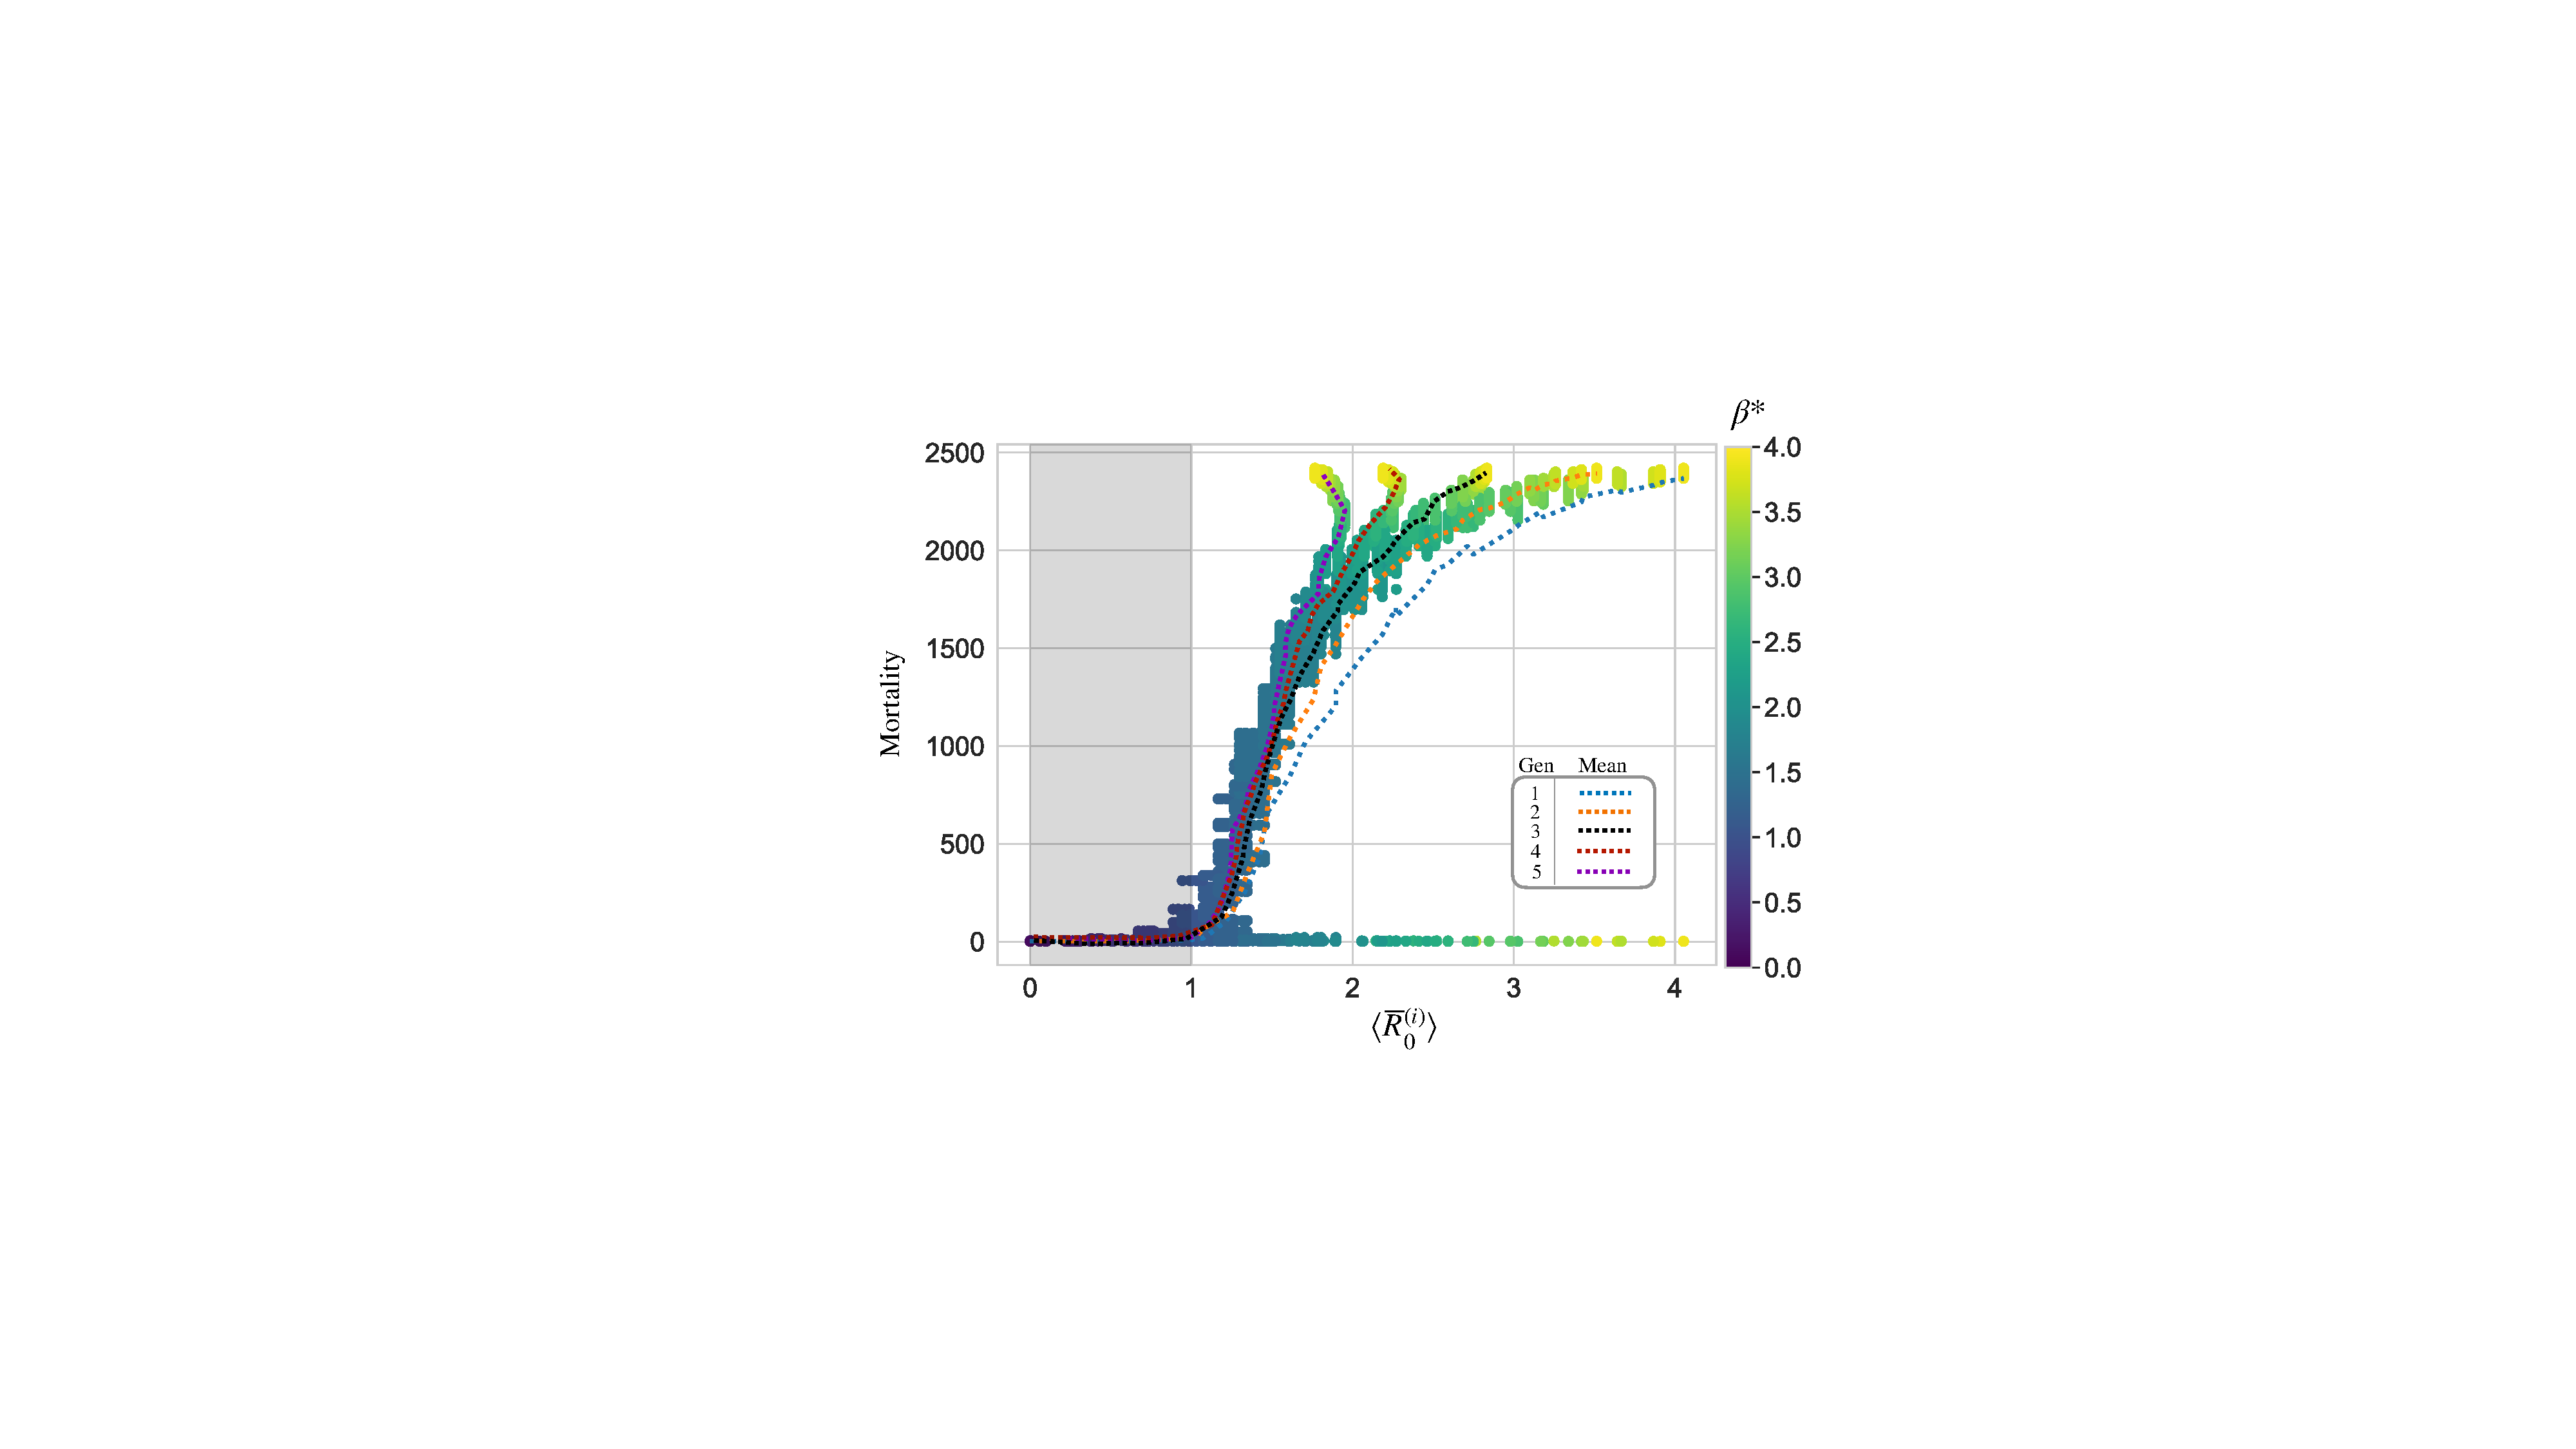
\includegraphics[scale=0.6]{chapter5/figures/fig6-R0-contact-vs-mortality.pdf}
    \caption{Contact-traced... \blindtext}
    \label{fig:contact-trace}
\end{figure}

% - Figures \ref{fig:contact-trace}(c-e) present a simple model to 
% - it is clear to see that methods of control should ideally target single high-priority links.
% - an assumption in and of itself)
\blindtext

\blindtext

\blindtext

\section{Chapter summary}

\blindtext

\blindtext

\blindtext

\blindtext

\newpage
